\makeatletter
\def\input@path{{../}}
\makeatother
\documentclass[../main.tex]{subfiles}

\begin{document}

\section{Introduction}% \label{sec:ising_intro}
%\todo[inline]{These are todonotes, in order to prevent them from showing up,
%comment out line 31 and uncomment line 30 in the tex file.} \comment{These are
%comments, in order to prevent them from showing up, comment out line 35 and
%uncomment line 34 in the tex file}
%
Machine learning (ML) is a general framework for recognizing patterns in data
without detailed human elaboration of the rules for doing so.
%
As an example, a very general function, with many parameters (for example,
thousands or millions) can be optimized on a training set, where the desired
output is known.
%
The problem is typically nonconvex and plagued by over-fitting problems, and so
advanced methods are necessary in order to get reliable answers.
%
One tool that has been exploited is principal component analysis (PCA), which
reduces the dimensionality of the data to the most important ``directions.''
Immediately the practitioner of renormalization group (RG) methods recognizes
an analogy, since the RG techniques are also supposed to identify the most
important directions in an enlarged space of Hamiltonians.
%
One of the motivations of the present research is to make this analogy more
concrete.

A number of papers~\cite{LiWang,Beny,MehtaSchwab} attempt to draw a connection
between deep learning and the RG as it appears in physics.
%
However, the analogies between RG flow and depth in a neural network would be
strengthened if one could determine conditions under which fixed points can be
identified.
%
It would be helpful to show more explicitly how passing from one level to
another in a neural network genuinely translates to a renormalization group
transformation.  There have been steps in the direction of making a full
connection.
%
For instance in~\cite{Beny}, the principle of \emph{causal influence} is
emphasized.
%
That is, when descending in depth, only neighboring nodes should influence the
outcome of a lower level node.
%
We have also implemented this in a simple training scheme in earlier
work~\cite{foreman2017}.
%
It can be called ``cheap learning'' because far fewer variational parameters
are involved, due to the constraints of locality.
% This can be viewed as a type of real space renormalization group. (Judah)
In~\cite{MehtaSchwab} it is emphasized that deep neural networks outperform
shallower networks for reasons which may ultimately be understood in terms of
the power of the renormalization group.
%
Other topics related to machine learning, such as principal component
analysis~\cite{BraddeBialek} have been previously interpreted in terms of the
renormalization group (in this case momentum shells).
%
Machine learning has also been used to identify phase transitions in numerical
simulations~\cite{2017NatPh..13..431C,PhysRevB.94.195105,2017PhRvE..95f2122H,2017PhRvE..96b2140W}.
%
RG transformations are usually defined in a space of couplings/Hamiltonians,
but typically, it is not possible to write down Hamiltonians directly
associated with image sets.
%
In this article we propose RG transformations that can be applied to a specific
set of images but which could be generalized for other image sets, and can also
be understood analytically without any graphical representation.
%
We use the well-studied example of the two-dimensional Ising model on a square
lattice.
%
The spin configurations generated with importance sampling provide images with
black and white pixels.
%
They have features that can be used to attempt to recognize the temperature
used to generate them. 
% there should be a citation here right?
%
However, constructing blocked Hamiltonians in configuration space is a
difficult task which involves approximations that are difficult to improve.
%
In other words, it is very difficult to explicitly construct the exact RG
transformation mapping the original couplings among the Ising spins into coarse
grained ones.
%

A better control on the RG transformation can be achieved by using the tensor
renormalization group (TRG)
method~\cite{PhysRevLett.99.120601,PhysRevB.79.085118,PhysRevB.86.045139,prb87,prd88,prd89,pre89}.
%
The starting point for this reformulation is the character expansion of the
Boltzmann weights which is also used in the duality
transformation~\cite{RevModPhys.52.453}.
%
This leads to an exact expression of the partition function as a sum over
closed paths which can be generated with importance sampling using the worm
algorithm~\cite{prok87} and then pixelated.
%
These samples will be our sets of images indexed by the temperature used to
generate them.
%
The procedure is reviewed in Sec.~\ref{configs_as_images}. 

The goal of a RG analysis is to study systems with large correlation lengths in
lattice spacing units and iteratively replace them by coarser ones with a
larger effective lattice spacing.
%
This process is useful if we can tune a parameter such as the temperature
towards its critical value.
%
Typical image sets such as the MNIST data can be thought as ``far from
criticality'' and the use of RG methods for such a data set may be of limited
interest~\cite{foreman2017}.
%
Criticality may sometimes refer to the choice of parameters used in data
analysis~\cite{PhysRevD.83.105014}. 
% do we mean to use refer here?  It seems crucial to introduce a systematic way
% to deal with the concept of criticality in ML. 

The PCA is a standard method to analyze sets of images.
%
In configuration space, the PCA analysis is identical to the study of the
spin-spin correlation matrix.
%
In particular, the largest eigenvalue $\lambda_{\mathrm{max}}$ is directly
connected to the magnetic susceptibility which diverges at
criticality~\cite{PhysRevB.94.195105}.
%
In the loop representation (worms), we will show that $\lambda_{\mathrm{max}}$
diverges logarithmically at criticality  with a constant of proportionality
which can be estimated quite precisely ($3/\pi$).
%
This is explained in Sec.~\ref{sec:pca}.
%
More generally, it seems reasonable to identify the criticality with the
divergence of $\lambda_{\mathrm{max}}$.

The advantage of rewriting the high-temperature expansion in terms of tensors
is that it allows a very simple blocking (coarse-graining) procedure where a
group of sites is replaced by a single site.
%
In the TRG approach the blocking procedure is local.
%
This leads to simple and exact coarse-graining formulas because we can separate
the links into two categories: those links that are inside the blocks and
integrated over, and those outside the blocks which are kept fixed and
communicate between the blocks~\cite{prb87}.
%
The main goal of this chapter is to relate blocking procedures that can be
applied to sets of pixelated images, to approximate TRG transformations.
%
A short summary of the TRG procedure is given in Sec.~\ref{sec:trg}.

Having defined criticality, the next step is to define a RG transformation for
sets of ``legal'' loop configurations, also called ``worm configurations''
later, sampled at various temperatures.
%
In Sec.~\ref{sec:rgimages},  we propose a family of transformations which
replaces two parallel links in a block by a single link carrying a specific
value $x$.  We call this procedure $1+1\rightarrow x$ hereafter.
%
In the case $1+1\rightarrow 0$, the blocked images follow the same rules (for
legal configurations) as the original ones.
%
There is a clear analogy with the 2-state approximation of the TRG method.
%
In the 2-state TRG approximation, the average fraction of occupied links shows
a characteristic crossing at a critical point and a collapse when the distance
to the critical point is appropriately rescaled at each iteration.
%
The average fraction of occupied links in the blocked worm configurations (with
$1+1\rightarrow 0$) shows a somewhat similar behavior in the low temperature
phase.
%
However, on the high-temperature side, we observe a ``merging'' rather than a
crossing.
%
In Sec.~\ref{sec:collapse},  we provide explanations for the similarities and
differences between the two procedures.

In Sec.~\ref{sec:nbtrg} we discuss an approximate 2-state TRG method to
calculate the average number of bonds through several iterations.
%
\begin{figure}[htpb]
    \centering 
    \includegraphics[width=0.5\textwidth]{aeye1.jpg}
    % \includegraphics[width=0.5\textwidth]{aeye1.jpg}%
    % \label{fig:aeye1}
    \hfill
    \includegraphics[width=0.5\textwidth]{aeye2.jpg}%
    % \label{fig:aeye2}%
    \hfill
    \includegraphics[width=0.5\textwidth]{beye.jpg}%
    % \label{fig:aeye3}%
    \hfill
    \caption{\label{fig:eye} (a) Picture of an eye with 4096 pixels; (b) black
    and white version with a graycut at 0.72; (c) boundaries of the black
    domains.}
\end{figure}
%
The worm configurations can be directly connected to spin configurations using
duality~\cite{RevModPhys.52.453}: they are the boundary of the positive spin
islands.
%
This suggests that the methods discussed here could be applied to generic
images.
%
Boundaries of generic grayscale pictures can be defined by converting the
picture to black and white pixels.
%
A grayscale picture with gray values between 0 and 1 can be converted into an
Ising spin configuration, by introducing a ``graycut'' below which the value is
converted to 0 (spin down) and above which the value is converted to 1 (spin
up).
%
It is then possible to construct the boundaries of the spin up domains.
%
This is illustrated in Fig.~\ref{fig:eye}.
%
Possible applications are briefly discussed in the Conclusions and illustrated
with the CIFAR database in Section~\ref{sec:cifar}. 

\section{From Loops to Images}%
\label{configs_as_images}

In the following we consider the two-dimensional Ising model with spins
$\sigma_i = \pm 1$ on a square lattice.
%
The partition function reads
%
\begin{equation}
  Z = \sum_{\{\sigma_i\}} e^{\beta \sum_{\langle i, j \rangle} \sigma_i
    \sigma_j}
\label{ih}, 
\end{equation}
%
where $\langle i, j \rangle$ denotes nearest neighbor sites on the square
lattice.
%
In some occasions we will use the notation $T=1/\beta$ for the temperature.
%
The partition function can be rewritten by using the character
expansion~\cite{RevModPhys.52.453}%\cite{prok87}%~\cite{prokofevIsing04}
%
\begin{equation}
\exp(\beta\sigma)=\cosh(\beta)+\sigma\sinh(\beta),
\end{equation}
%
and integrating over the spins.
%
Factoring out the $\cosh(\beta)$, each link can carry a weight 1 when
unoccupied or $t\equiv \tanh(\beta)$ when occupied.
%
The integration over the spins guarantees that an even number of occupied links
is coming out of each site~\cite{RevModPhys.52.453}.
%
The set of occupied links then form a ``legal graph'' with $N_b$ occupied
links.
%
The partition function can then be written as sum over such legal graphs. If
$\mathcal{N}(N_b)$ denotes the number of legal graphs with $N_b$ links we can
write: 
%
\begin{equation}
    Z=2^V{(\cosh(\beta))}^{2V}\sum_{N_b} t^{N_b}\mathcal{N}(N_b).
\label{eq:nbsum}
\end{equation}
%
Using the fact that $\tanh(\beta)=\exp(-2\tilde{\beta})$, with $\tilde{\beta}$
the inverse dual temperature, Eq.~(\ref{eq:nbsum}) has the same form as a
spectral decomposition using a density of states and a Boltzmann weight (with
$2N_b$ playing the role of the energy).
%
Details of this reformulation can be found in
Section~\ref{ssec:loop_representation}.

As shown in Section~\ref{ssec:heat_capacity}, we can use derivatives of the
logarithm of the partition function to relate $\langle N_b\rangle$ to the
average energy, and the bond number fluctuations,
%
\begin{equation}
\label{eq:fluc}
\langle \Delta_{N_b}^2 \rangle \equiv \langle{\left(N_b - \langle
  N_b\rangle\right)}^2\rangle,
\end{equation}
%
to the specific heat per site. From the logarithmic singularity of the specific
heat we find that 
%
\begin{equation}
    \langle \Delta_{N_b}^2\rangle /V =-\frac{2}{\pi}\ln(|T-T_c|)+{\rm regular}.
    \label{eq:specific_heat_fluctuation_eq2}
\end{equation}
%
In the following we use interchangeably the ``bond'' terminology, for instance
in $N_b$ as in~\cite{prok87} and the link terminology more common in the
lattice gauge theory context.
%
In all our numerical simulations we use periodic boundary conditions which
guarantees translation invariance.
% \comment{Periodic boundary conditions are used for all numerical simulations
% in order to guarantee translational invariance. (rewrite?)}

We will show in Sec.~\ref{sec:trg} that the new form of the partition function
in Eq.~(\ref{eq:nbsum}) can also be written in an equivalent way as a sum of
products of tensors with four indices contracted along the links of the
lattice.

The contributions to Eq.~(\ref{eq:nbsum}) can be sampled using a worm
algorithm~\cite{prok87} outlined in
Section~\ref{ssec:monte_carlo_implementation}.
%
Using this algorithm, we generated multiple configurations at each temperature
($N_{\mathrm{configs}} \approx10,000$) which are then used for averaging.
%
For example, we can calculate the average number of occupied bonds at a
particular temperature by averaging over all configurations.

Using a legal graph (worm configuration), we can construct an image by
introducing a lattice of $2L\times2L$  pixels with a size of one half lattice
spacing.  One quarter of these pixels are attached to the sites, one quarter to
the horizontal links and one quarter to the vertical links. The remaining
quarter are in the middle of the plaquettes and always white.  In this
representation, each site, link, and plaquette are designated an individual
pixel, where occupied links and their respective endpoints are colored black.
An example of this representation is shown in
Fig.~\ref{fig:worm_as_image}.
%
\begin{figure*}[htpb]
 \centering
 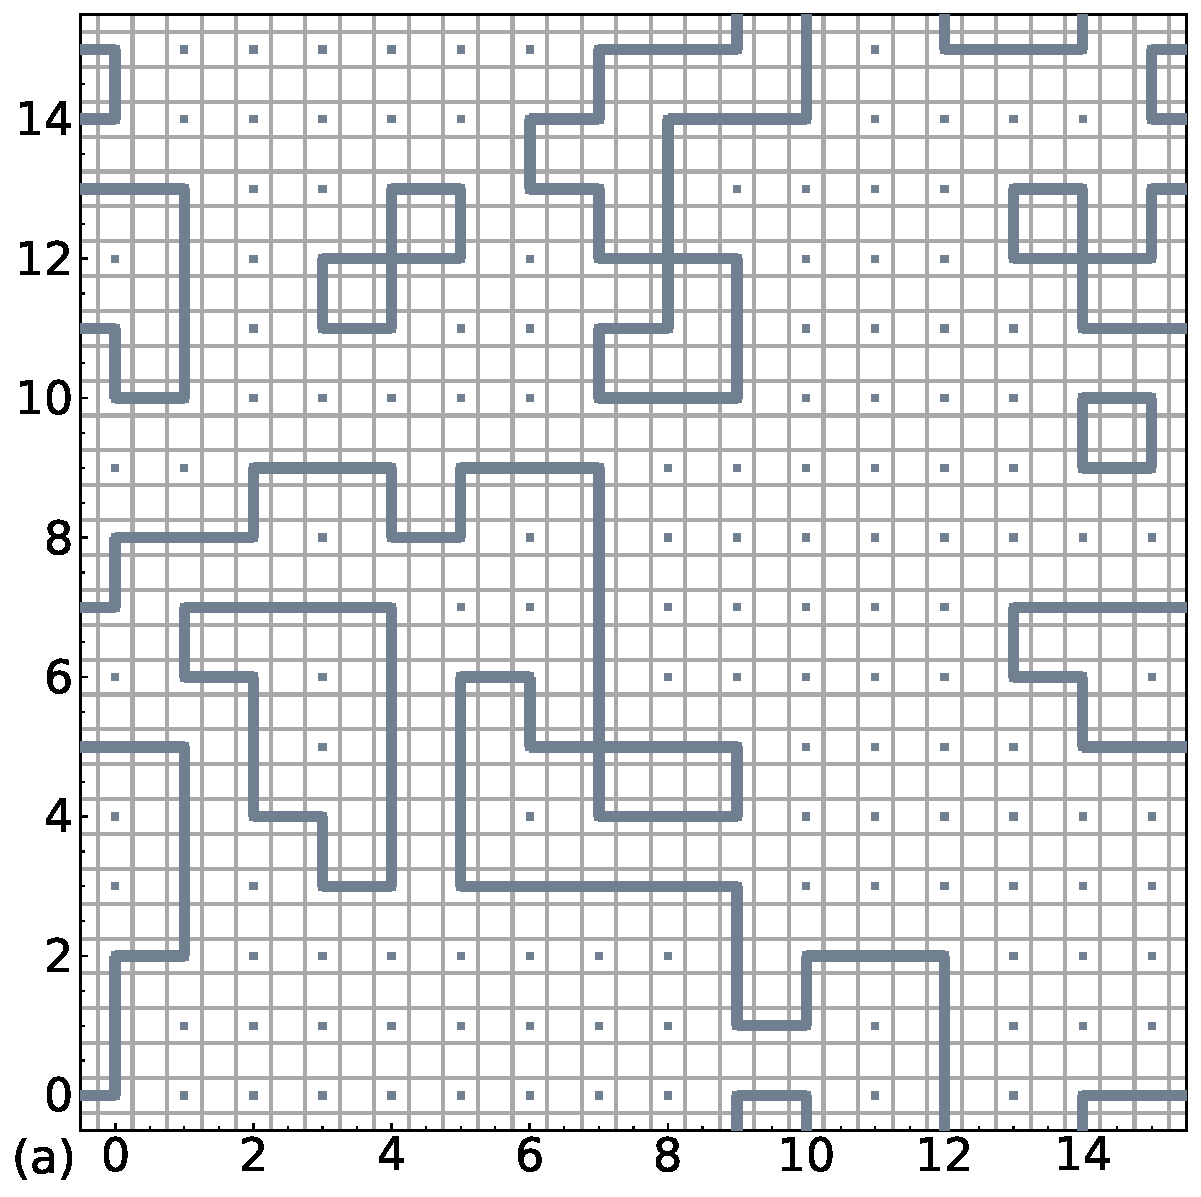
\includegraphics[width=0.49\textwidth]{worm_configuration_16_unblocked_grid.pdf}
 \hfill
 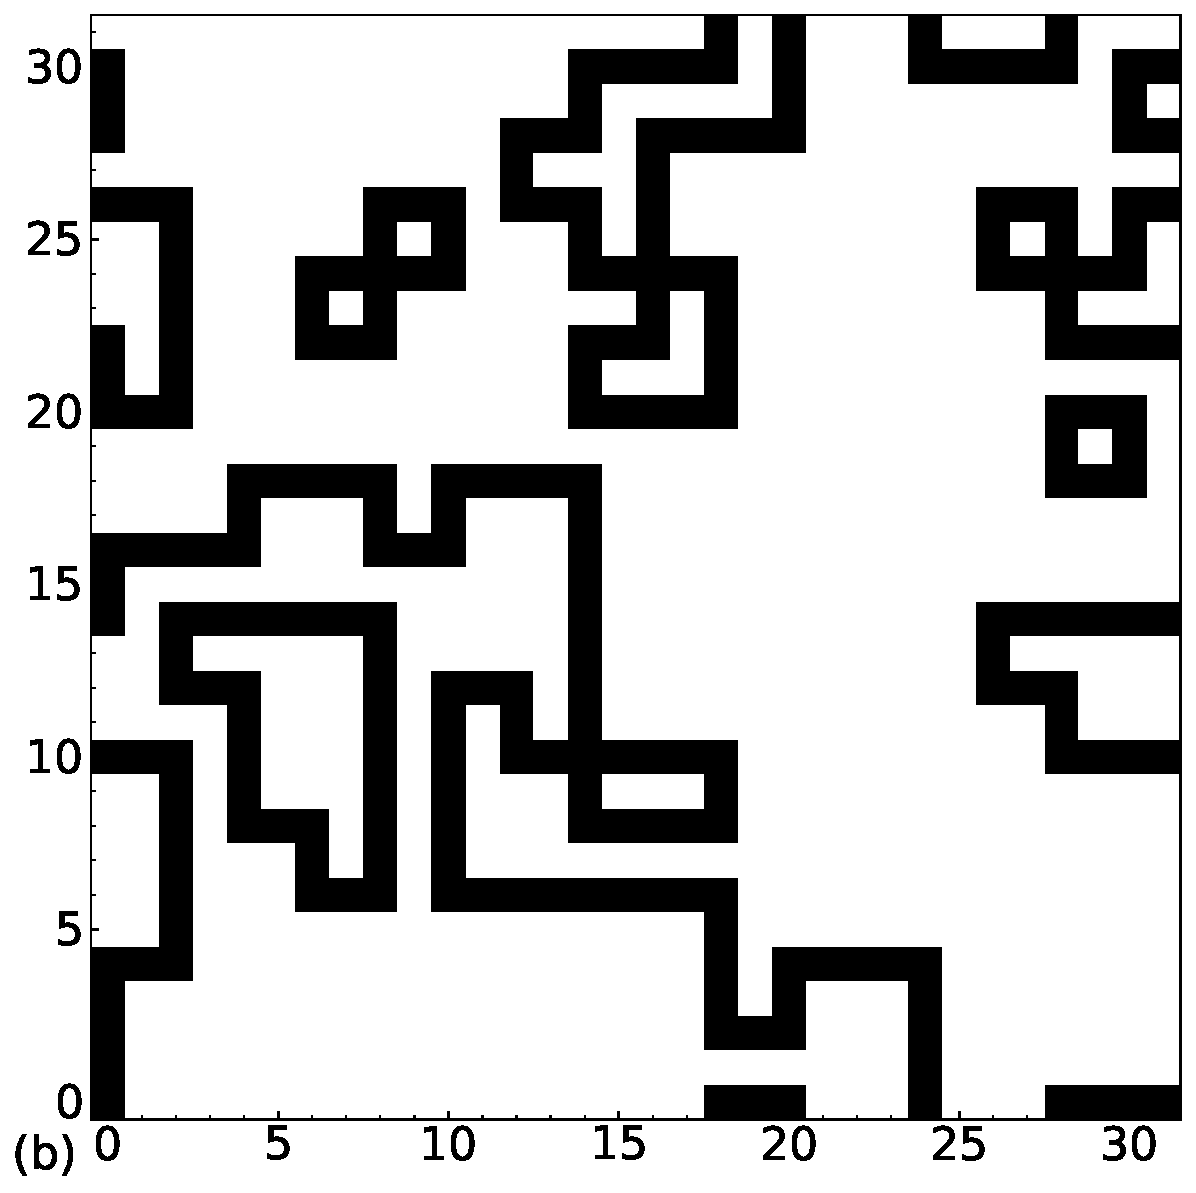
\includegraphics[width=0.49\textwidth]{worm_configuration_16_unblocked_image.pdf}
 \caption{(a) Legal worm configuration on an $L \times L$ lattice with periodic
		boundary conditions and; (b) its equivalent representation as a
		$2L\times2L$ black and white pixel image.}%
 \label{fig:worm_as_image}
\end{figure*}
%
We can then flatten each of these images into a vector $\mathbf{v} \in
\mathbb{R}^{4V}$, with $v_i \in \{0, 1\}$.
%
This allows us to write the number of occupied bonds, in a single
configuration, $N_b$ as
%
\begin{equation}
    \sum_{j = bonds} v_j = N_b
    \label{eq:link_sum}
\end{equation}
%
\section{PCA and Criticality}%
\label{sec:pca}
Having now sets of images for a range of temperatures, we can apply
PCA~\cite{Bishop}.
%
PCA isolates the ``most relevant'' directions in the dataset.
%
PCA is simply the computation of the eigenvalues $\lambda_\alpha$ and
eigenvectors $u_\alpha$ of the covariance matrix for a dataset with $N$
configurations corresponding to a given temperature ${\{{\bf v}^n\}}_{n=1}^N$:
%
\begin{equation}
S_{ij} = \frac{1}{N} \sum_{n=1}^N (v_{i}^n - {\bar v}_i)
(v_{j}^n - {\bar v}_j).
\end{equation}
%
In this equation, each sample ${\bf v}_j$ is a vector in $\mathbb{R}^{4V}$,
labeled by the indices $i,j = 1,\ldots,4V$.
%
The PCA extracts solutions to
%
\begin{equation}
S u_\alpha = \lambda_\alpha u_\alpha
\end{equation}
%
and orders them, in descending magnitude of $\lambda_\alpha$, which are all
non-negative.
%
The usefulness of PCA is that one can approximate the data (see for instance
the discussion in~\cite{Bishop}) by the first $M$ principal components. 

Illustrations of the PCA for the MNIST data can be found in Sec.~4 of
Ref.~\cite{foreman2017}, where we show the eigenvectors corresponding to the
largest eigenvalues and the approximation of the data by subspaces of the
largest eigenvalues of dimensions 10, 20 etc. 

It should be noted that the PCA is an analysis that can be performed for each
temperature separately and not obviously connected to the closeness to
criticality.
%
However, we were able to find a relation between the largest PCA eigenvalue
denoted $\lambda_{\max}$ and the logarithmic divergence of the specific heat,
namely
%
\begin{equation}
    \lambda_{max} \simeq \frac{3}{2}\left \langle \Delta_{N_b}^2
    \right\rangle/V\simeq -\frac{3}{\pi}\ln(|T-T_c|).
    \label{eq:eigval_delta_Nb}
\end{equation}
%
This property was found by an approximate reasoning shown in
Section~\ref{ssec:heat_capacity} and relies on two assumptions.
%
The first one is that the eigenvector associated with $\lambda_{max}$ is
proportional to $\langle \mathbf{v}\rangle$ which is invariant under
translation by two pixels in either direction.
%
The second assumption is that in good approximation we can neglect the
contributions from sites that are visited twice (four occupied links coming out
of one site).
%
Numerically, only 4\% of sites are visited twice near the critical temperature
which justifies the second assumption.
Figure~\ref{fig:eigval_fluctuations_unblocked} provides an independent
confirmation of the approximate validity of Eq.~(\ref{eq:eigval_delta_Nb}). 
%
\begin{figure}[htpb]
 \centering
 % 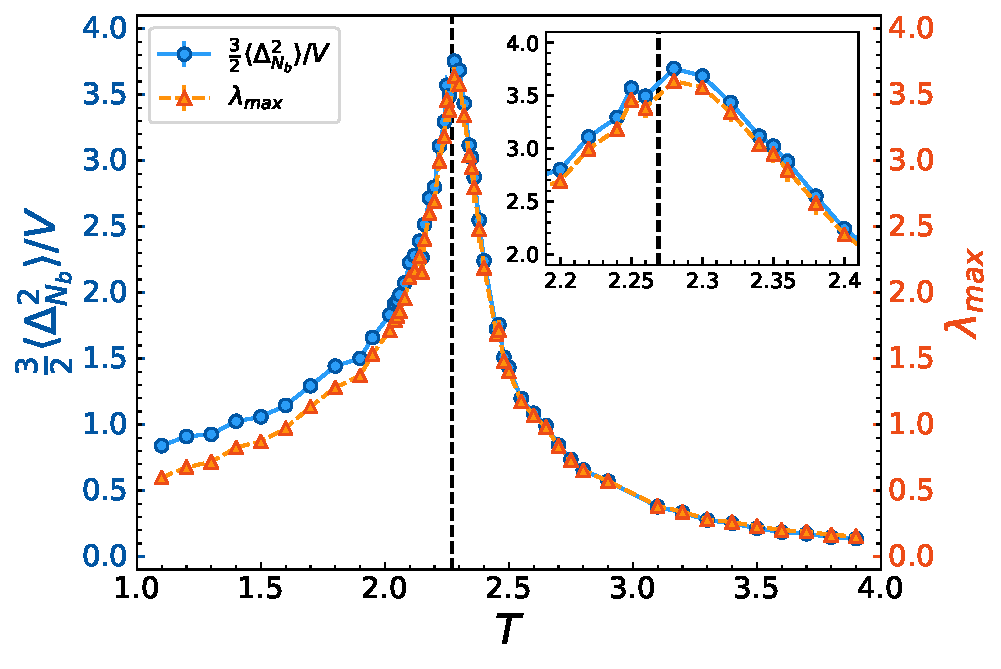
\includegraphics[width=17.2cm]{delta_Nb_lambda_max_compare_inset}\hfill
 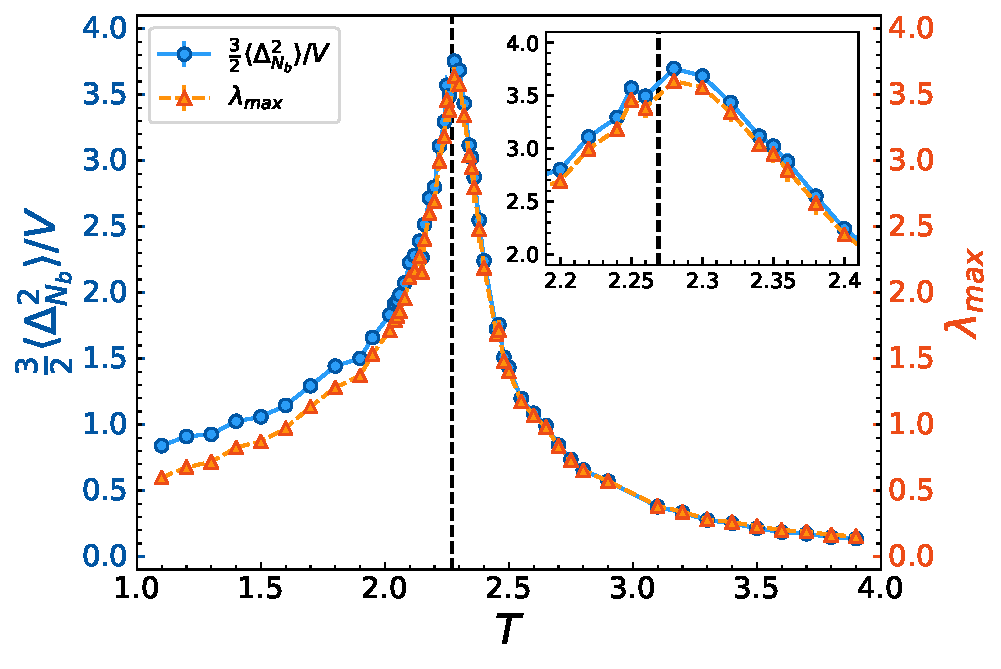
\includegraphics[width=0.8\textwidth]{delta_Nb_lambda_max_compare_inset}
	\hfill
 \caption{$\lambda_{max}$ and $\frac{3}{2}\left \langle \Delta_{N_b}^2
		\right\rangle / V$ (per unit volume) vs. $T$, illustrating the relation
		between the eigenvalue corresponding to the first principal component and
		the logarithmic divergence of the specific heat. The inset shows a
		qualitative agreement near the critical temperature.}%
 \label{fig:eigval_fluctuations_unblocked}
\end{figure}
%
\section{TRG Coarse-graining}%
\label{sec:trg}
So far we  have sampled the legal graphs of the high temperature expansion of
the Ising model using the worm algorithm.
%
An alternative approach is to use a tractable real-space renormalization group
method known as the TRG~\cite{PhysRevB.86.045139,prb87,prd88,prd89,pre89}. 

In order to understand what we want to accomplish by blocking the \lc
configuration, it is useful to first understand the evolution of a tensor
element using the TRG method. 

The tensor formulation used here connects easily with  the worm formulation
used in this paper.
%
After the character expansion has been carried out, one is left with new
integer variables on the links of the lattice with constraints on the sites
which guarantee the sum of the link variables associated with that site is
even.
%
Therefore we build a tensor using this constraint and the surrounding link
weights.
%
The tensor has the form
%
\begin{equation}
    T^{(i)}_{x\xp y\yp}(\beta) = 
    {\left[\tanh(\beta)\right]}^{(n_{x}+n_{\xp}+n_{y}+n_{\yp})/2}
    \times \delta_{n_{x}+n_{\xp}+n_{y}+n_{\yp}\,\mathrm{mod}\,2,\,\,0}.
\end{equation}
% \begin{eqnarray} T^{(i)}_{x x' y y'}(\beta)& =
% &[\tanh(\beta)]^{(n_{x}+n_{x'}+n_{y}+n_{y'})/2}\\ &\
% &\delta_{n_{x}+n_{x'}+n_{y}+n_{y'}, 0\text{ mod }2}.  \end{eqnarray}

Here the notation being used is that this tensor is located at the
$i$\textsuperscript{th} site of the lattice, $n_{\hat{\mu}}$ is the integer
variable, taking value 0 or 1, on an adjacent link, and the Kronecker delta,
$\delta_{i,j}$ is understood to be satisfied if the sum is even.
%
By contracting these tensors together in the pattern of the lattice one
recreates the closed-loop paths generated by the high-temperature expansion and
exactly match those paths which are sampled by the worm algorithm.

Using these tensors one can write a partition function for the Ising model that
is exactly equal to the original partition function,
%
\begin{equation}
 Z =2^V {(\cosh (\beta))}^{2V}\Tr \prod_{i}T^{(i)}_{x\xp y\yp} 
\end{equation} 
%
where $\Tr$ means contractions (sums over 0 and 1) over the links. 

The most important aspect of this reformulation is that it can be
coarse-grained efficiently.
%
The process is illustrated in Fig.~\ref{fig:unit_block} where four fundamental
tensors have been contracted to form a new ``blocked'' tensor.  This new tensor
has a squared number of degrees of freedom for each new effective index. The
partition function can be written exactly as 
%
\begin{equation*}
  Z= 2^V{(\cosh (\beta))}^{2V}\Tr\prod_{2i}T^{\prime\,
    (2i)}_{XX^{\prime}YY^{\prime}} \ , 
\label{eq:ZP}
\end{equation*}
%
where $2i$ denotes the sites of the coarser lattice with twice the lattice
spacing of the original lattice. 
%
\begin{figure}[htpb]
    \centering
    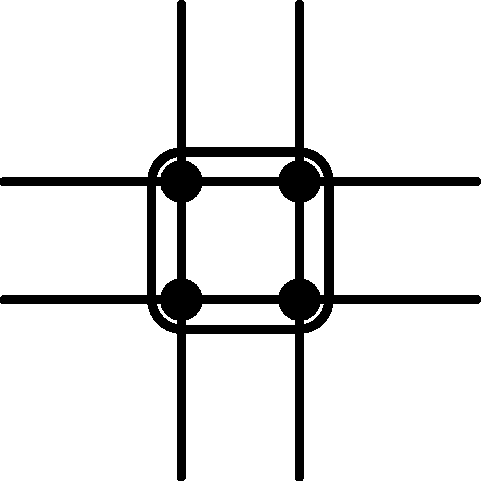
\includegraphics[width=0.45\textwidth]{blocked-1.pdf}
    \caption{Illustration of the tensor blocking discussed in the text.  Each
      dot is a tensor at a lattice site with four lines coming out, each
      representing a tensor index.  Lines connecting dots represent tensor
    contractions.}%
\label{fig:unit_block}
\end{figure}
%
In practice, this exact procedure cannot be repeated indefinitely and
truncations are necessary.
%
This can be accomplished by projecting the product states into a smaller number
of states that optimizes the closeness to the exact answer.
%
A two-state projection is discussed in~\cite{prb87} and will be followed
hereafter.
%
Note that in this procedure, $T_{0000}$ is factored out and the final
expression for the other blocked tensors are given in these units.
%
For definiteness we consider $T_{1100}$ which in the microscopic formulation is
the weight associated with a horizontal line in a \lc configuration.
%
By looking at the fixed point equation~\cite{prb87}, one can see that there is
a high temperature fixed point where all the tensor elements except for
$T_{0000}$ are zero and a low temperature fixed point where all the tensor
elements are one.
%
In between these two limits, there is a non-trivial fixed point illustrated by
the crossing of iterated values of $T_{1100}$ in Fig.~\ref{fig:T1100}. Note
that because of the two-state approximation, the critical temperature $T_c$ is
slightly higher than the exact one~\cite{prb87}.
%
To be completely specific, the exact $T_c$ for the original model is
$2/\ln(1+\sqrt{2})=2.269\ldots$ while for the two state projection with the
second projection procedure of Ref.~\cite{prb87}, it is $1/0.3948678
=2.53249\ldots$
%
\begin{figure*}[htpb]
	\centering 
	 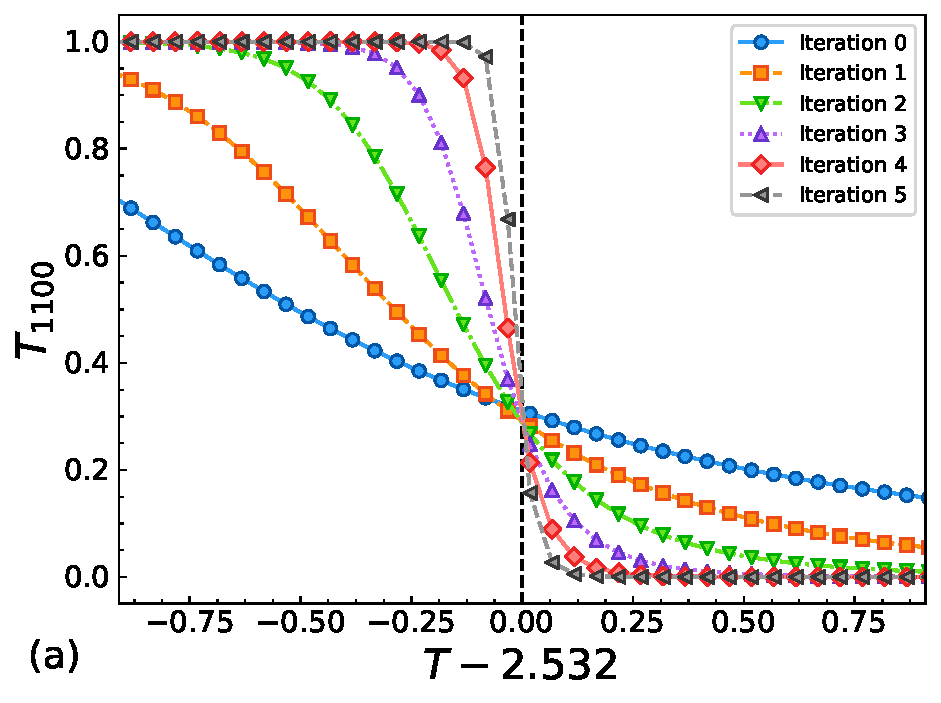
\includegraphics[width=0.49\textwidth]{trg_T1100_vs_T}
	 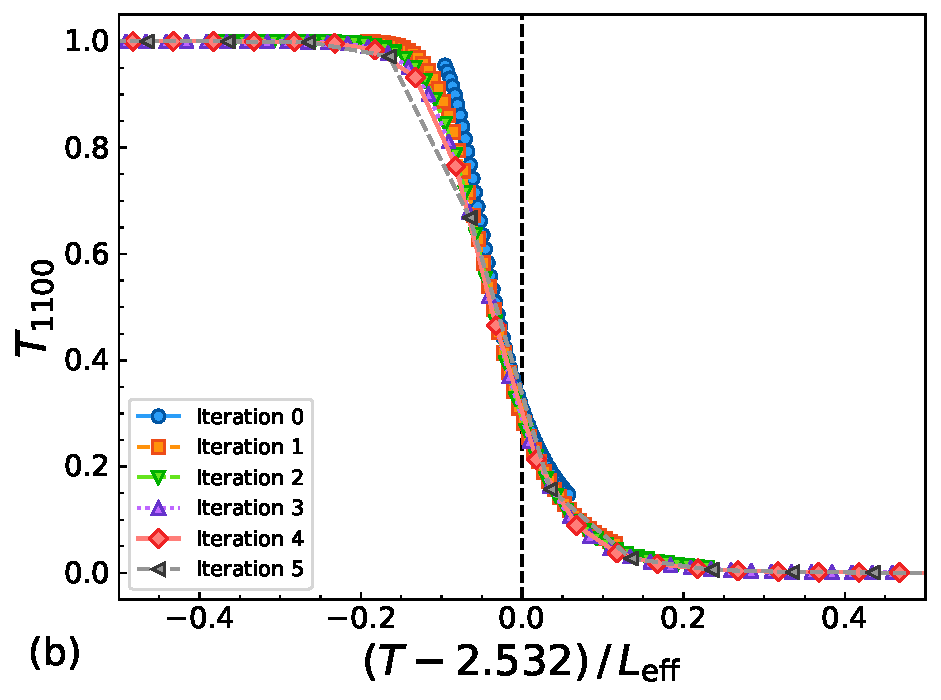
\includegraphics[width=0.49\textwidth]{trg_T1100_vs_T_collapsed}
	 \caption{(a) $T_{1100}$ vs. $T - T_c^{(2s)}$ for six successive iterations
		 of the blocking transformation, beginning with an initial lattice $L =
		 64$; (b) $T_{1100}$ vs. $(T - T_{c}^{(2s)}) / L_{\mathrm{eff}}$
		 illustrating the data collapse, where $T_{c}^{(2s)}$ is the critical
		 temperature of the two state projection, beginning at iteration 0 on an
		 $L = 64$ lattice.}%
\label{fig:T1100}
\end{figure*}
%
It is easy to relate the properties of the iterated curves near the non-trivial
fixed point using the linear RG approximation.
%
Below we just state the results, for details and references see~\cite{prb87}.
With the blocking procedure used, the scale factor is $b=2$.
%
The eigenvalue in the relevant direction is $\lambda=b^{1/\nu}=2$ since
$\nu=1$. In Fig.~\ref{fig:T1100} (a), one can see that the height
%
\begin{equation}
    \delta T_{1100} \equiv T_{1100} - T_{1100}^{*}
\end{equation}
%
(where $T_{1100}^{*}$ is the value at the fixed point), nearly doubles each
time the blocking procedure is performed, making the slope twice as large each
time.
% In Fig.~\ref{fig:T1100}, one can see that near $T_c$, the height with respect
% to the crossing point nearly doubles each time, making the slope twice bigger
% each time.
A nice data collapse can be reached by offsetting this effect by rescaling the
horizontal axis each iteration by $\lambda$=2 as shown in Fig.~\ref{fig:T1100}
(b).
%
In numerical calculations, we start with a finite $L$ (64 in
Fig.~\ref{fig:T1100}) and then after $\ell$ iterations, we are left with an
effective size $L_{\mathrm{eff}}=L/b^\ell$. 

The remainder of this chapter will be dedicated towards obtaining data collapse
for $\langle N_b \rangle$ calculated with successive blockings.

\section{Image Coarse-graining}%
\label{sec:rgimages}
In an attempt to explicitly connect the ideas from RG theory to similar
concepts in machine learning, we will implement a coarse-graining procedure
directly on the images but in a way inspired by the TRG construction of
Sec.~\ref{sec:trg}.
%
The construction relies on visual intuition and will be reanalyzed in the TRG
context in Sec.~\ref{sec:nbtrg}.

% As in the TRG coarse graining we divide the original into blocks of $2\times2$
% squares, reducing the size of each linear dimension by a factor of two.
As in the TRG coarse-graining procedure, the image is first divided up into
blocks of $2\times2$ squares, as shown in Fig.~\ref{fig:blocked-2}.
%
\begin{figure}[htpb]
    \centering
    \includegraphics[width=\textwidth]{lattice_cg.png}
    \caption{Illustration of the coarse-graining procedure in which the
      original lattice sites ($i$) are replaced by blocked sites ($2i$) (grey
      circles) with twice the original lattice spacing. In the coarse-grained
      lattice, an elementary block (blue) consists of four sites on the
      original lattice, eight external bonds (red), and four blocked external
      bonds (green).}%
\label{fig:blocked-2}
\end{figure}
%
Each of these $2\times2$ squares are then replaced, or ``blocked'', by a single
site with bonds determined by the number of occupied external bonds in the
original square.
%
In doing so, we reduce the size of each linear dimension by a factor of two,
resulting in a new blocked configuration whose volume is one-quarter the
original.
%
In particular, if a given block has exactly one external bond in a given
direction, the blocked site retains this bond in the blocked configuration.
%
This seems to be a natural choice.
%
However, if a given block has exactly two external bonds in a given direction,
we can consider several options. The simplest option is to neglect the double
bond entirely, and we denote this blocking scheme by ``$1+1\rightarrow 0$''.
%
This approach respects the selection rule (conservation modulo 2) and has the
advantage of maintaining the closed-path restriction.
%
In other words with the $1+1\rightarrow0$ option, the blocked image corresponds
to a legal graph and the procedure can be iterated without introducing new
parameters.
%
This procedure is illustrated for a specific configuration on a $16\times16$
lattice in Fig.~\ref{fig:110}.
%
\begin{figure*}[htpb]
    \centering
    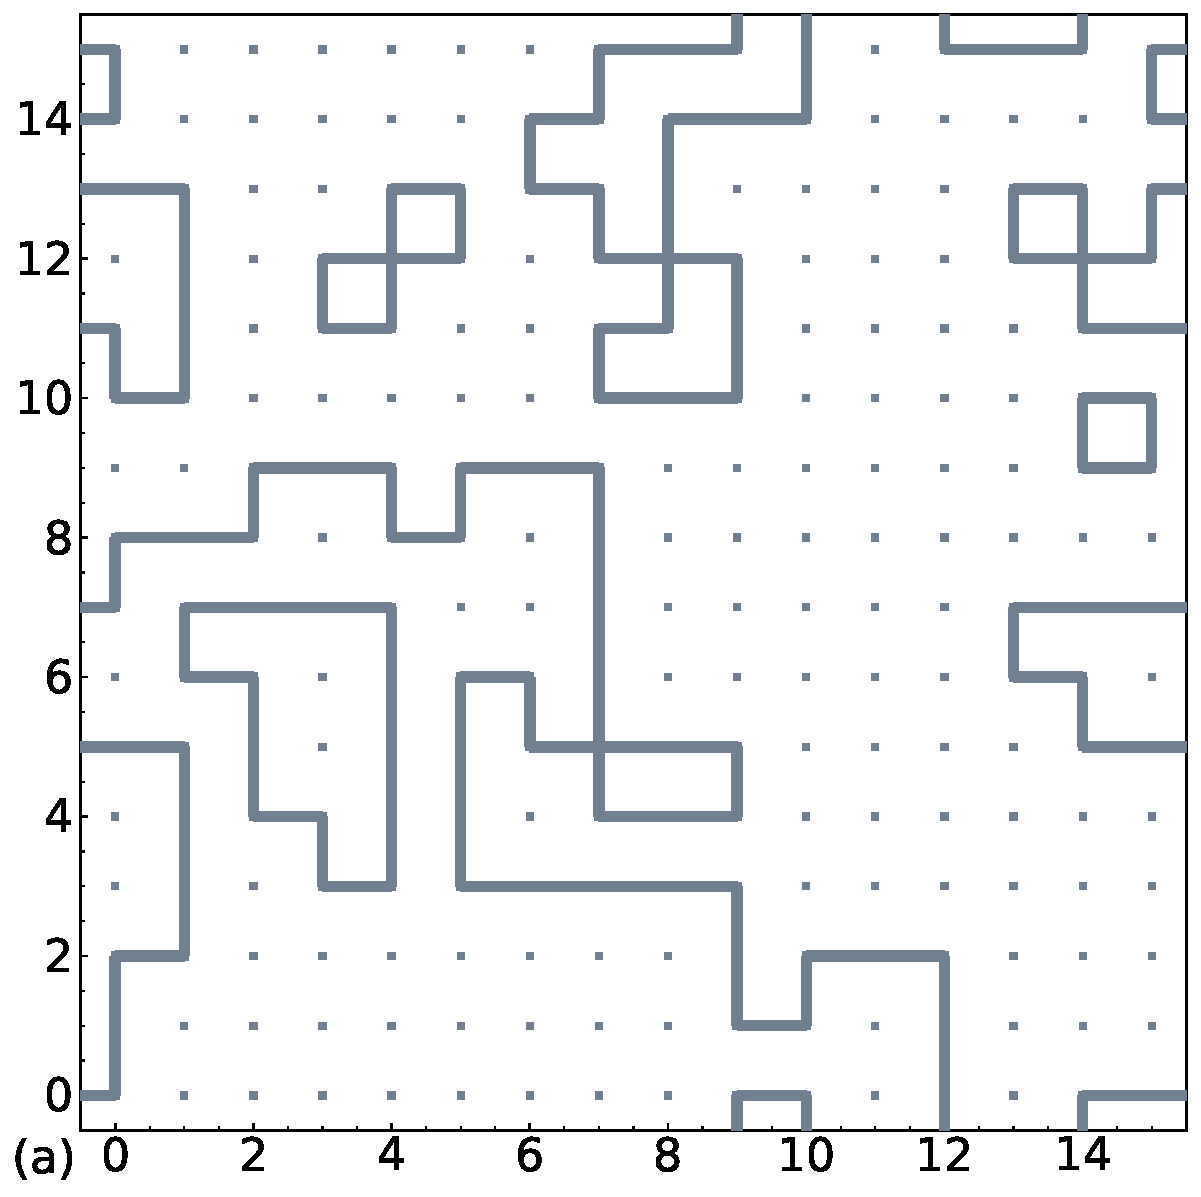
\includegraphics[width=0.33\textwidth]{worm_configuration_16_unblocked}\hfill%
    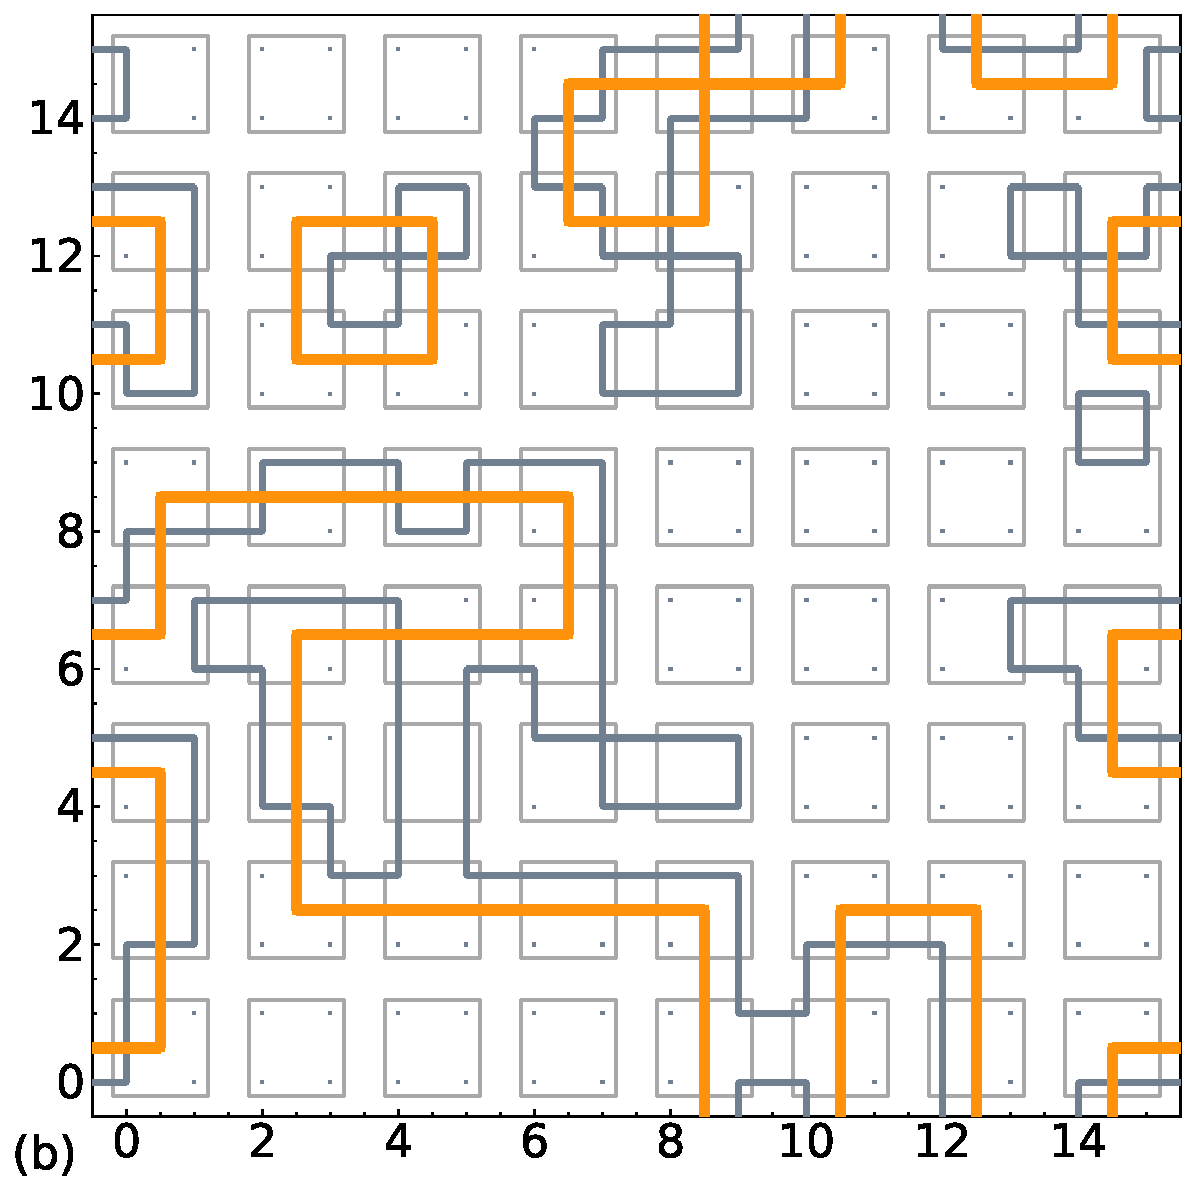
\includegraphics[width=0.33\textwidth]{worm_configuration_16_blocked110}\hfill%
    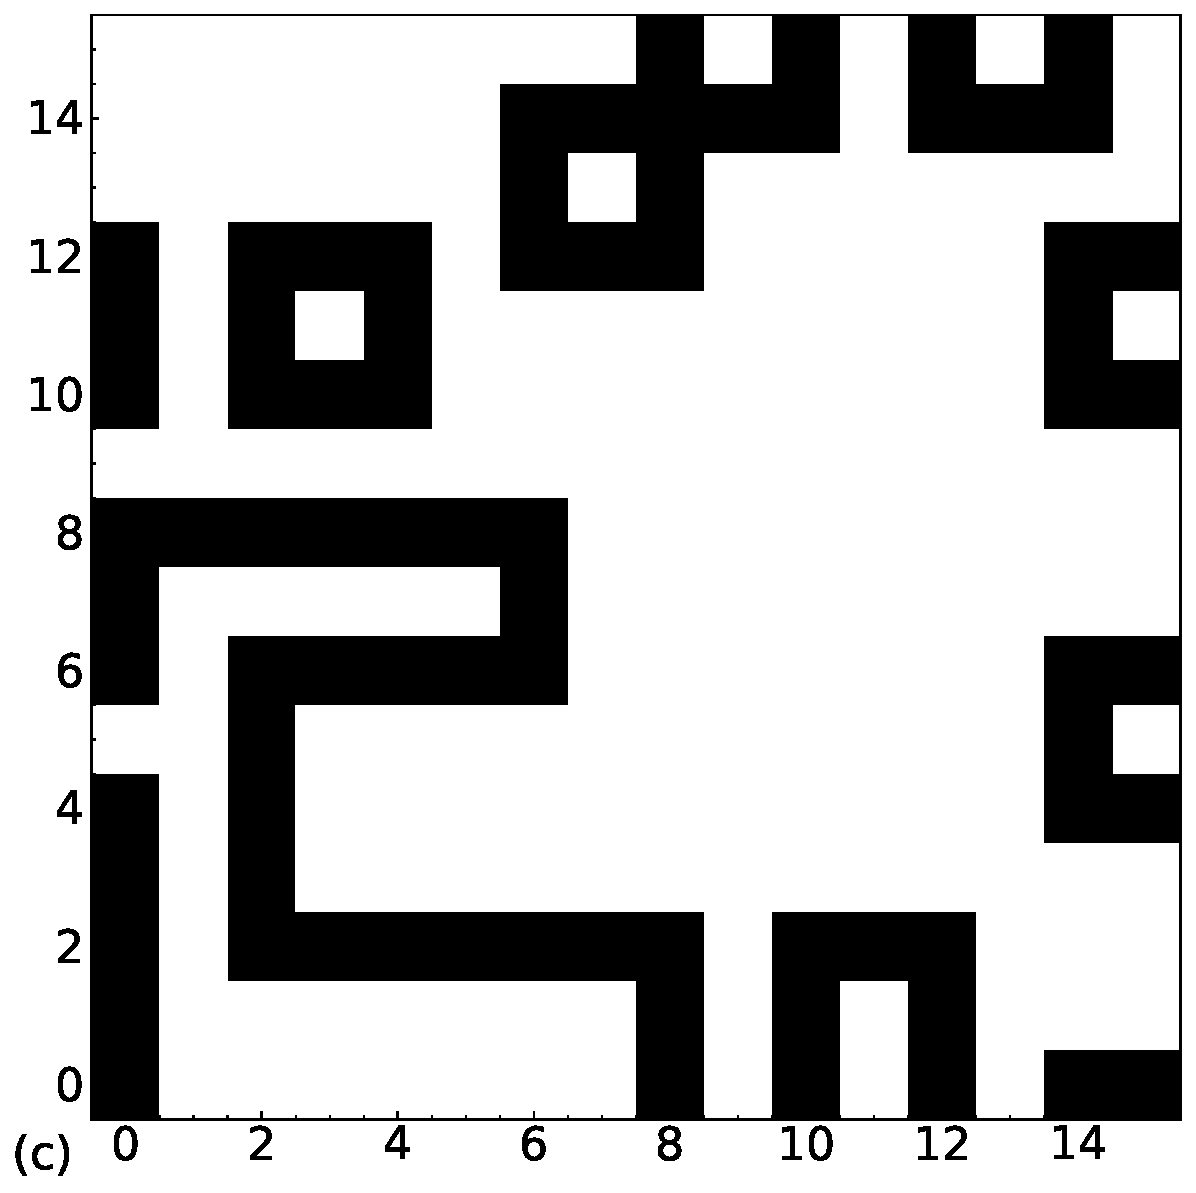
\includegraphics[width=0.33\textwidth]{worm_configuration_16_blocked110_image}
    \caption{(a) Illustration of the $1+1\rightarrow 0$ blocking
        procedure discussed in the text: original configuration; (b)
        introduction of the blocks and replacement of single or double bounds
        according to the $1+1\rightarrow 0$ rule; (c) construction of the
    corresponding  blocked image.}%
\label{fig:110}
\end{figure*}
%
Alternatively, we can include this double bond in the blocked configuration,
and give it some weight $m$ between 0 and 2.
%
The examples of $m=$ 1 and 2 are denoted ``$1+1\rightarrow 1$'', and
``$1+1\rightarrow 2$'' respectively and are shown in
Fig.~\ref{fig:double_bond_weights}.
%
This blocking procedure introduces new elements and iterations require more
involved procedures.
%
This is not discussed hereafter. 

\section{Partial Data Collapse for Blocked Images}%
\label{sec:collapse}
In this section, we study the properties of $\langle N_b\rangle$  obtained for
successive blockings with the $1+1\rightarrow0$ rule starting with
configurations on a $64\times64$ lattice.
%
A first observation is that the $1+1\rightarrow0$ blocking preserves the
location of the peak of the fluctuations $\langle\Delta_{N_b}^2\rangle$.
%
 In addition it is possible to stabilize this quantity for a few iterations by
dividing by $V_{\mathrm{eff}}\ln(L_{\mathrm{eff}})$.
%
This is illustrated in Fig.~\ref{fig:delta_Nb_iterated}.
%
However, a very different scaling appears for the last two iterations which may
be due to the very short effective sizes (4 and 2).
%
This indicates the last two iterations are very different from the previous
ones. 
%
\begin{figure}[htpb]
    \centering
    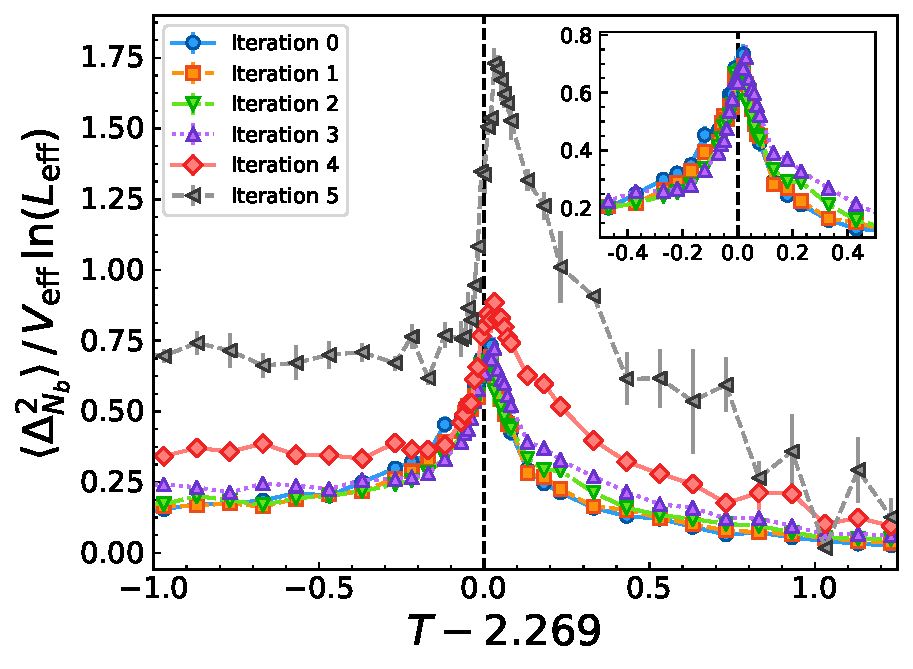
\includegraphics[width=\textwidth]{delta_Nb_iterated}\hfill
    \caption{Fluctuations in the average number of bonds $\langle
      \Delta_{N_b}^2\rangle$ vs.\ temperature $T$ under iterated blocking steps
      beginning with an initial lattice size of $L = 64$. The results are
      scaled by $1 / V_{\mathrm{eff}}\log(L_{\mathrm{eff}})$ in order to
      demonstrate the data collapse near the critical temperature. This
      collapse is especially apparent in the inset, which shows the results
      under the first three blocking steps, with $L_{\mathrm{eff}} = 64, 32,
      16$, and $8$.}%
\label{fig:delta_Nb_iterated}
\end{figure}
%
We now consider $\langle N_b\rangle$ for successive iterations.
%
The results are shown in Fig.~\ref{fig:imagecollapsed}.
%
We see that in the low temperature side, the curves sharpen in a way similar to
$T_{1100}$ in Fig.~\ref{fig:T1100}.
%
However on the high temperature side, we observe a merging rather than a
crossing.
%
This can be explained as follows.
%
In the high T regime occasionally a single loop, the size of a plaquette,
forms.
%
This is due to other configurations being highly suppressed.
%
With the $1+1\rightarrow0$ rule, one out of four possible plaquettes becomes a
larger plaquette which exactly compensates the change in $V_{\mathrm{eff}}$
which is also reduced by a factor of four.
%
There are four kinds of plaquettes (see Fig.~\ref{fig:110}): those inside the
blocks (they disappear after blocking), those between two neighboring blocks in
the vertical or horizontal direction (these are double links between the blocks
and so they disappear with the $1+1\rightarrow0$ rule), and finally those which
share a corner with four blocks (they generate a larger plaquette).
%
This last type can be seen at coordinate (4, 12) in Fig.~\ref{fig:110}.
% illustrations can be found near (4,12) in Fig.~\ref{fig:110}.
%
\begin{figure*}[htpb]
    \centering 
    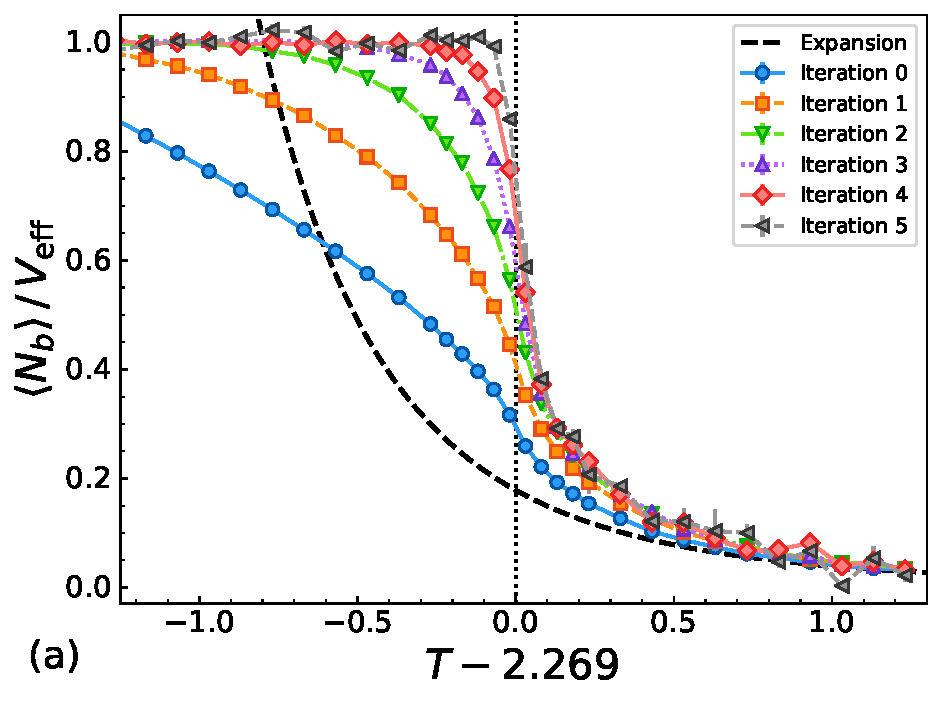
\includegraphics[width=0.49\textwidth]{Nb_avg_iterated_with_expansion}\hfill%
    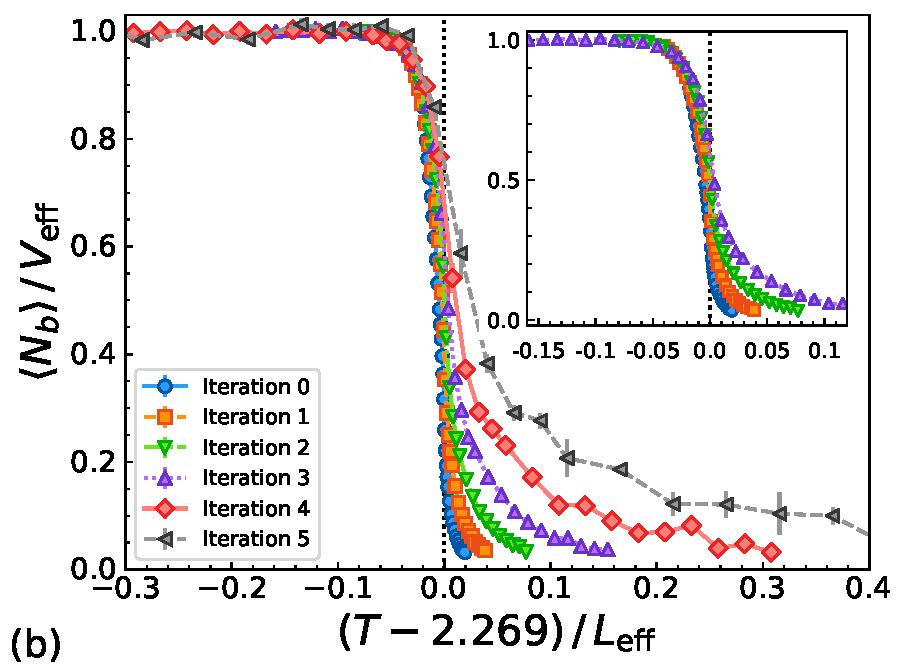
\includegraphics[width=0.49\textwidth]{Nb_avg_iterated_collapsed}
    % 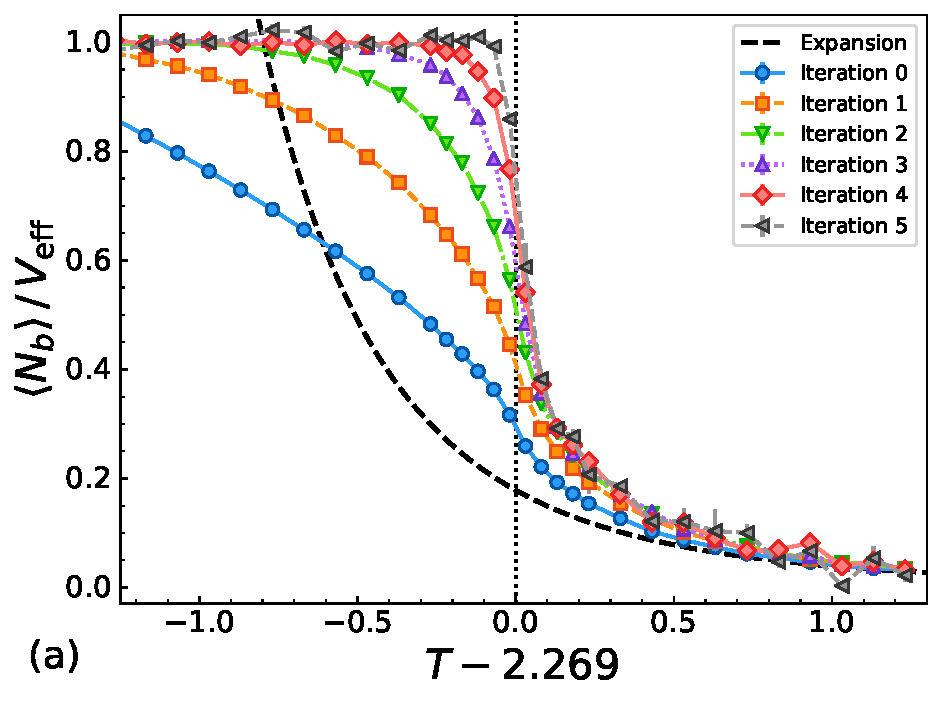
\includegraphics[width=0.45\textwidth]{Nb_avg_iterated_with_expansion}
    % 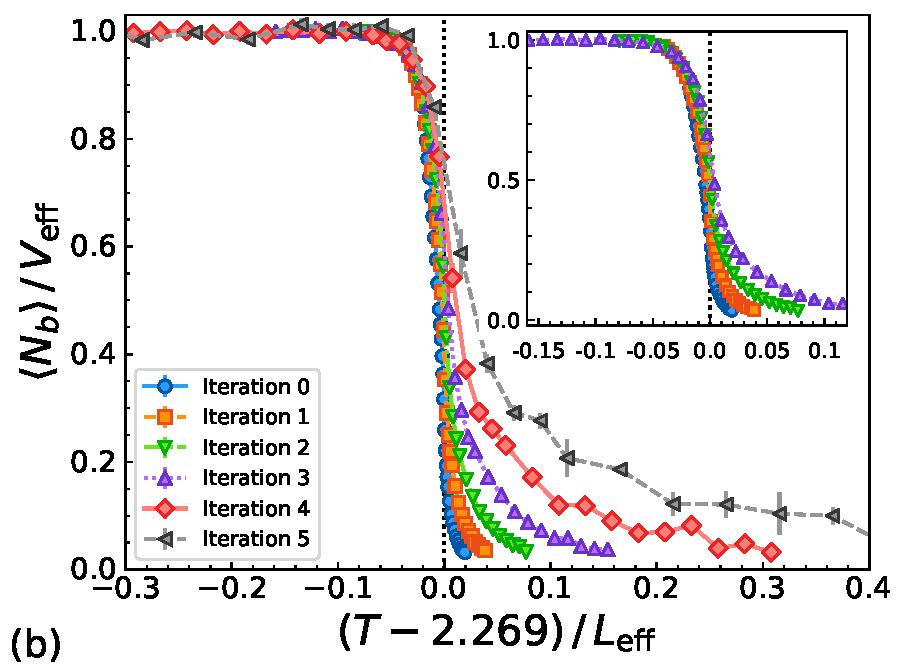
\includegraphics[width=0.45\textwidth]{Nb_avg_iterated_collapsed}
    \caption{(a) Average number of bonds $\langle N_b\rangle$ vs.\ temperature
      $T$ under iterated blocking steps beginning with an initial lattice size
      of $L = 64$. The dashed black line illustrates the high temperature
      expansion, showing that the dominant configurations are those consisting
      of small, isolated plaquettes. (b) Average number of bonds $\langle
      N_b\rangle$ vs.\ the rescaled temperature $(T - 2.269) /
      L_{\mathrm{eff}}$ under successive blocking steps. Iteration 0 represents
      the original lattice before blocking, with $L_{\mathrm{eff}} = 64$. }%
\label{fig:imagecollapsed}
\end{figure*}
%
We now attempt to obtain data collapse for $\langle N_b \rangle/V_{eff}$ by
performing a rescaling of the temperature axis with respect to the critical
value as in Fig.~\ref{fig:T1100}.
%
After this rescaling by a factor 2 at each iteration, we observe a reasonable
collapse on the low-temperature side.
%
On the high temperature side, since the unrescaled curves merge, the rescaling
splits them and there is no collapse on that side.
%
This is illustrated in Fig.~\ref{fig:imagecollapsed}.  

\section{TRG Calculation of \texorpdfstring{$\langle N_b \rangle$}{<Nb>}}%
\label{sec:nbtrg}
Using the tensor method we were able to calculate $\langle N_{b} \rangle$ to
compare with the worm algorithm.
%
Consider the equation for $\langle N_{b} \rangle$ with $N_{b} = \sum_{l} n_{l}$
the sum over bond numbers at every link:
%
\begin{equation}
    \langle N_{b} \rangle = \frac{1}{Z} \sum_{\{n\}} \left( \sum_{l} n_{l}
    \right) \left( \prod_{l} \tanh^{n_{l}}(\beta) \right){\left(
    \prod_{i}
    \delta^{(i)}_{n_{x}+n_{\xp}+n_{y}+n_{\yp}\,\mathrm{mod}\,2,\,\,0}\right)}.
\end{equation}
%
This expression can be seen as $\langle N_{b} \rangle = \sum_{l} \langle n_{l}
\rangle$, and because of translation and $90^{\circ}$ rotational invariance,
all $\langle n_{l} \rangle$ are equal.
%
Thus, it is enough to calculate
$\langle n_{l} \rangle$ for one particular link (just call it $\langle
n\rangle$) and multiply it by $2V$: $\langle N_{b} \rangle = 2V \langle n
\rangle$.

To calculate $\langle n \rangle$, it amounts to associating an $n$ with one
particular link on the lattice.
%
This alters \emph{two} tensors on the lattice such that the two tensors which
contain that link as indices are now defined as
%
\begin{align}
	\tilde{T}^{(1)}_{n_{x} n_{\xp} n_{y} n_{\yp}}  &=
    \sqrt{n_{x}} T_{n_{x} n_{\xp} n_{y} n_{\yp}} (\beta),\\
    \tilde{T}^{(2)}_{n_{x} n_{\xp} n_{y} n_{\yp}}  &=
    \sqrt{n_{\xp}}T_{n_{x} n_{\xp} n_{y} n_{\yp}} (\beta),
\end{align}
%
where $x$ and $\xp$ were chosen without loss of generality.
%
It could just as well have been chosen as $y$ and $\yp$.
%
One can see that when these two tensors are contracted along their shared link,
the product picks up a factor of $n$ for that link, which when combined with
the other tensors in the lattice, and divided by $Z$, yields $\langle n
\rangle$.

Knowing the above, one is free to block and construct the partition function,
$Z$, and $\langle n \rangle$.
%
This can be done by blocking symmetrically in both directions, or by
constructing a transfer matrix by contracting only along a time-slice (i.e.\ a
snapshot of the system at fixed $t$).
%
This is shown in Fig.~\ref{fig:tm}.
%
In practice contracting to build a transfer matrix is optimum since one
direction of the lattice is never renormalized and allows the easy calculation
of $\langle n \rangle$.
%
\begin{figure}[htpb]
 \centering
 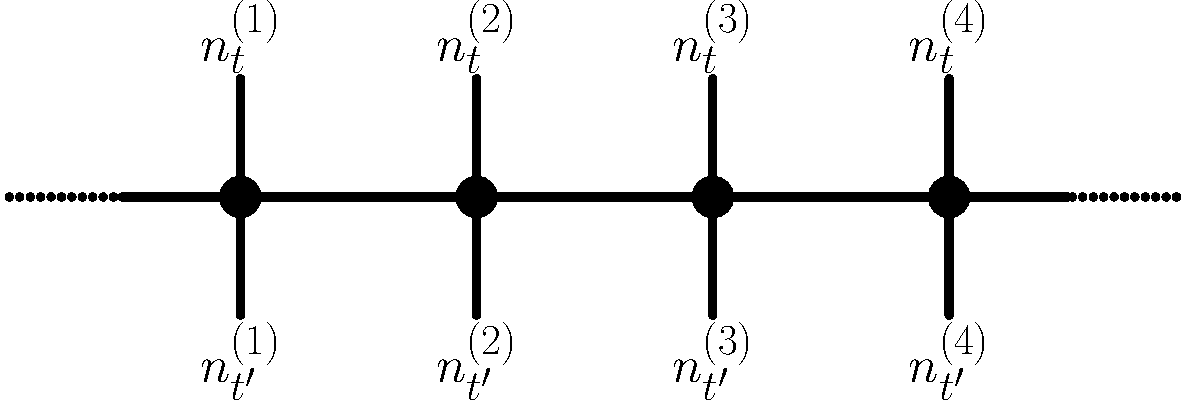
\includegraphics[width=0.6\textwidth]{tm-1.pdf}
 \caption{A pictorial representation of the transfer matrix made by
	 contracting a fundamental tensor along a single time-slice.}%
\label{fig:tm}
\end{figure}
%
%
What was just described is a method to calculate $\langle n \rangle$ for the
original, fine lattice.
%
However, one can also calculate the same quantity for a coarse lattice.
%
The actual blocking method is essentially identical, with a small difference.
%
Instead of contracting the fundamental tensor to the desired lattice size, one
contracts a blocked tensor to the desired lattice size.

For example, if one wanted to calculate $\langle N_{b} \rangle$ for a $32
\times 32$ lattice, one could contract the fundamental tensor along a time
slice with itself five times.
%
This would give a $2^{32} \times 2^{32}$ transfer matrix which could be used to
build the whole partition function.
%
Now, under a single coarse-graining step the $32\times 32$ lattice becomes a
$16\times 16$ lattice of blocks.
%
Therefore, to build this, one could contract four fundamental tensors in a
block and consider this a new, effective fundamental tensor.
%
This is shown in Fig.~\ref{fig:unit_block}.
%
Then one repeats the same steps to construct the transfer matrix, however only
contracting four times with itself to create a matrix representing 16 lattice
sites of the blocked tensor.

To actually calculate $\langle n \rangle$ by building the transfer matrix, one
can take the final tensor, prior to contracting the dangling spatial indices,
and multiply by $\sqrt{n}$ against the indices $n_{x}$ and $n_{\xp}$.
%
This is shown for the unblocked case in Fig.~\ref{fig:nb}, however the
procedure is identical for the blocked case once the blocked tensor has been
constructed.
%
\begin{figure}[htpb]
  \centering
	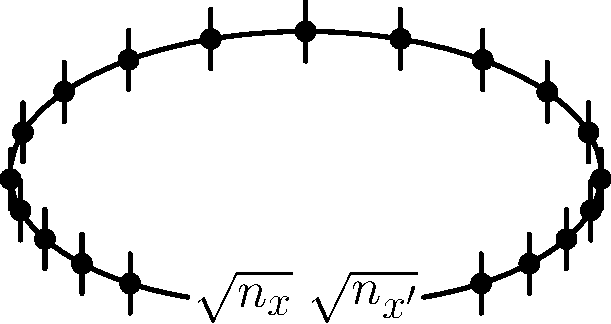
\includegraphics[width=0.6\textwidth]{nb_insert-1.pdf}
    \caption{By multiplying the remaining free spatial indices by $\sqrt{n}$
    and contracting for periodic boundary conditions in space we form an
    ``impure'' transfer matrix.  Combining the resultant matrix with the
    original transfer matrix allows one to calculate $\langle n \rangle$.}%
\label{fig:nb}
\end{figure}
%
This is also the point where one can choose the level of approximation one will
use in the blocking.
%
For instance one could choose that the state $|1 \; 1 \rangle \rightarrow
|0\rangle$ and assign $n = 0$ to that state.
%
Alternatively one could preserve $N_{b}$ and let $|1 \; 1 \rangle \rightarrow
|2 \rangle$ and assign $n = 2$ to that state.
%
This procedure was found to agree with the results obtained by changing the
pixels of the worm configurations.

Once the original transfer matrix has been constructed, as well as the matrix
with the insertion of $n$ along a single link, one can combine these to find
$\langle n \rangle$.
%
This is done by simple matrix multiplication:
%
\begin{equation}
    \langle n \rangle = \frac{1}{Z} \Tr[\underbrace{\mathbb{T} \cdots
    \mathbb{T}^{\prime} \cdots \mathbb{T}}_{N_{\tau}}],
\end{equation}
%
with
%
\begin{equation}
	Z = \Tr[\mathbb{T}^{N_{\tau}}].
\end{equation}
%
Here $\mathbb{T}$ represents the transfer matrix built by contracting tensors
along a time slice, and $\mathbb{T}^{\prime}$ represents the single
(``impure'') transfer matrix at a time-slice with a single bond multiplied by
$n$.
%
Since the lattice has Euclidean temporal extent, $L = N_{\tau}$, there are that
many matrices multiplied in each case.
%
The values of $\langle N_b\rangle/V_{\mathrm{eff}}$ obtained with this
procedure are shown in Fig.~\ref{fig:Nb_2s_HOTRG}.
%
The rescaling by 2 at each iteration provides a good data collapse on both
sides of the transition.
%
\begin{figure*}[htpb]
    \centering 
    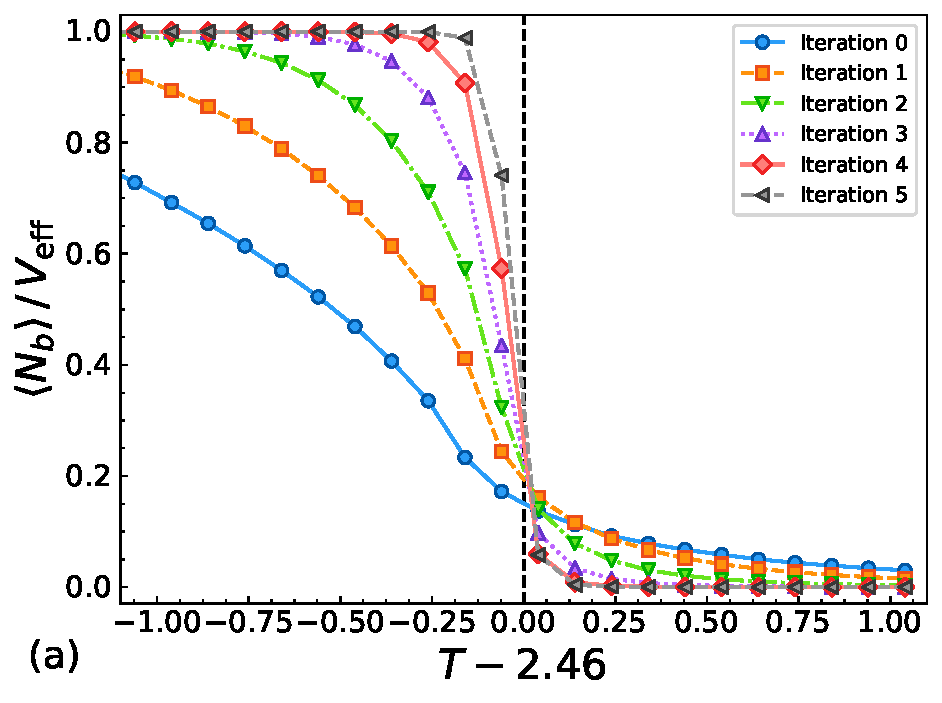
\includegraphics[width=0.49\textwidth]{Nb_2sHOTRG_5iter}\hfill%
    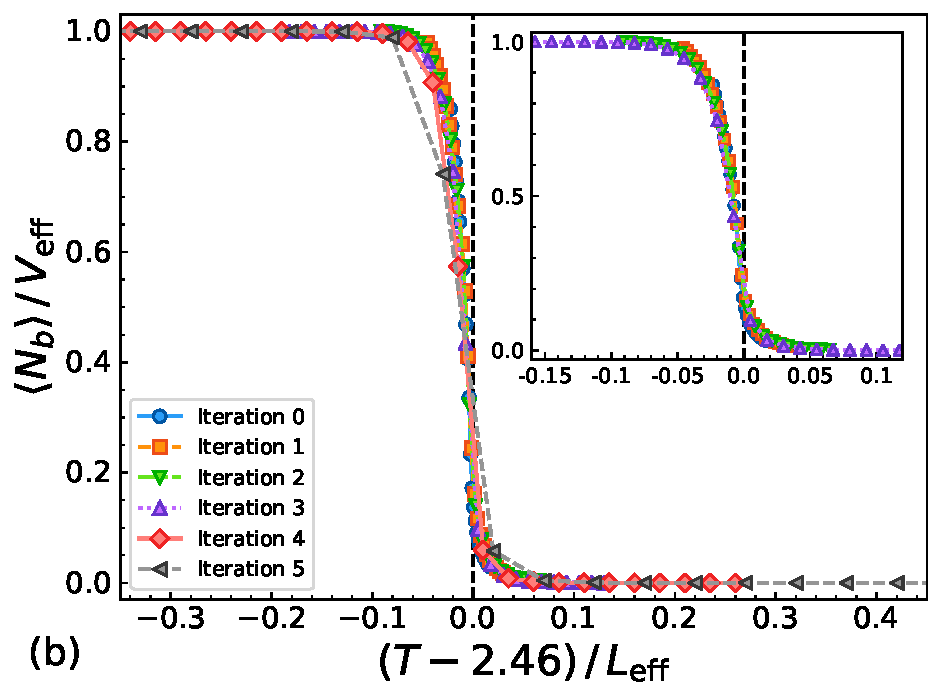
\includegraphics[width=0.49\textwidth]{Nb_2sHOTRG_5iter_collapsed}
    \caption{(a) $\langle N_b\rangle$ vs $(T - 2.46)$ under successive blocking
      steps calculated using 2-state HOTRG.\@ (b) $\langle N_b\rangle$ vs $(T -
      2.46) / L_{\mathrm{eff}}$ under successive blocking steps calculated
      using 2-state HOTRG.\@ Note that the value of $2.46$ was determined
      qualitatively by choosing the value which gave the best resulting data
      collapse.}%
\label{fig:Nb_2s_HOTRG}
\end{figure*}
%
\section{Technical Results}%
\label{sec:technical_results}
\subsection{Loop Representation}%
\label{ssec:loop_representation}
We can rewrite the Ising partition function in terms of bonds between
neighboring sites $\langle i , j \rangle$.
%
The allowed bond configurations are concisely described by concepts in graph
theory, because they form edges (bonds) between neighboring vertices (sites).
%
Making use of well-known identities allows for the partition function to be
written in the following high-temperature expansion:
%
\begin{align}
    Z &= 2^{|V|} \cosh^{|E|} \beta \sum_{\Gamma \in {\cal C}(G)}
			\tanh^{|\Gamma|}(\beta) \\
		&= 2^{|V|} \cosh^{|E|} \beta \sum_{|\Gamma|} n(|\Gamma|)
			\tanh^{|\Gamma|}(\beta)
\label{eq:z}
\end{align}
%
The notation is as follows.
%
We have a graph $G=(V,E)$ that describes our lattice, where $V$ are the
vertices and $E$ are the edges, which are the bonds between neighboring sites.
%
If we restrict ourselves to subgraphs with only occupied bonds allowed by the
Ising model, then the degree of each vertex is even.
%
This is the number of bonds emanating from a particular vertex.
%
The set of edges of such a subgraph is described as being ``Eulerian.''
%
The space of all such sets of edges is known as the cycle space ${\cal C}(G)$.
%
The notation $|V|$, $|E|$, $|\Gamma|$ denotes the number of elements in each
set (cardinality).
%
In the second line, $n(|\Gamma|)$ counts the multiplicity of subgraphs of
cardinality $|\Gamma|$, and is zero when $|\Gamma|$ does not correspond to a
``legal'' subgraph.

We now specialize the presentation to the case of the two-dimensional Ising
model on a square lattice with periodic boundary conditions.
%
In this case $|V|$ is $V=L^2$, the volume that we express in lattice units, and
$|E| = 2V$.
%
We introduce the notation $t\equiv\tanh(\beta)$ and we call $N_b$ the number of
bonds in a graph (values taken by $|\Gamma|$).
%
With these notations we recover Eq.~\ref{eq:nbsum}.

It is this bond formulation that is the basis of both random cluster
algorithms~\cite{Swendsen:1987ce} and worm algorithms~\cite{prok87}.
%
In this paper we utilize the latter.
%
Both of these classes of algorithms have the benefit of significantly avoiding
critical slowing down.
%
This is essential near the critical temperature $T_c$.

\subsection{Heat Capacity}%
\label{ssec:heat_capacity}
One striking feature of the second order transition for the two-dimensional
Ising model is the logarithmic divergence of the specific heat density at the
critical temperature $T_c$.
%
In this section, we review the way the specific heat can be calculated with the
worm algorithm and we check our answer with the exact finite volume
expressions~\cite{bkaufman}.

Using the standard thermodynamical formula for the average energy
%
\begin{equation}
    \langle E \rangle = - \frac{\partial}{\partial \beta} \ln Z,
\end{equation}
%
with the expression Eq.~(\ref{eq:nbsum}) of  $Z$, we get
%
\begin{equation}
    \langle E \rangle = - \tanh(\beta)\left(2V + \frac{\langle
    N_b\rangle}{\sinh^2(\beta)}\right),
\end{equation}
%
where we define
%
\begin{equation}
\langle f(N_b)\rangle \equiv \sum_{N_b} f(N_b)t^{N_b}  n(N_b)/\sum_{N_b}t^{N_b}
n(N_b).
\end{equation}
%
We can then use
%
\begin{equation}
    C_{V} = \frac{\partial \langle E \rangle}{\partial T},
\end{equation}
%
to write
%
% \begin{align}
\begin{equation}
  \frac{C_V}{V} = \beta^2 {\left[\frac{2}{\cosh^2(\beta)} 
      - \frac{4\cosh(2\beta)}{\sinh(2\beta)}
      \frac{\langle N_b\rangle}{V}
      + {\left(\frac{2}{\sinh(2\beta)}\right)}^2\frac{\langle{(N_b 
  - \langle N_b\rangle)}^2\rangle}{V} \right]}.
\end{equation}
% \end{align}
%
%Singularity of $C_V$ at $T = T_C$
Since $\frac{\langle N_b\rangle}{V}\leq 2$ (in two dimensions), the only
possibly divergent part is the variance of $N_b$ per unit volume $\langle
\Delta_{N_b}^2\rangle$ defined in Eq.~(\ref{eq:fluc}).
%
The singularity near $T_c$ is known from Onsager's solution:
%
\begin{equation}
    \frac{C_V}{V} = -\frac{2}{\pi}{\left(\ln(1+\sqrt{2})\right)}^2
    \ln{\left(|T - T_c|\right)} + \text{regular}.
    \label{eq:onsager}
\end{equation}
%
This implies Eq.~(\ref{eq:specific_heat_fluctuation_eq2}).  
%
\subsection{Monte Carlo Implementation}%
\label{ssec:monte_carlo_implementation}
We can proceed to sample the closed path configuration space using the worm
algorithm~\cite{prok87}.
%
A single Monte Carlo step is outlined below.
%
\begin{enumerate}
    \item Randomly select a starting point on the lattice $(i_0, j_0)$.
    \item Propose a move to a neighboring site $(i^{\prime}, j^{\prime})$,
        selected at random.
    \item If no link is present between these two sites, a bond is created with
        acceptance probability $P = \min\{1, \tanh{\beta}\}$. If the bond is
        accepted, we update the bond number for the present worm, $n_b = n_b +
        1$.
    \item If a link already exists between the two sites, it is removed with
        probability $P = 1$.
    \item If $(i^{\prime}, j^{\prime}) = (i_0, j_0)$, i.e.\ we have a closed
        path, go to (1.). Otherwise, $(i^{\prime}, j^{\prime}) \neq (i_0,
        j_0)$, go to (2.)
\end{enumerate}
%
The number of necessary Monte Carlo steps required to achieve sufficient
statistics varies with the lattice size, thermalization time, and temperature.
%
After each step, we calculate the energy in terms of the average number of
active bonds $N_b$, and consider the system to be thermalized when fluctuations
between subsequent values of the energy are less than $1\times10^{-3}$.
%
We then save the resulting configuration, along with the final values for all
physical quantities of interest.
%
This process is then repeated many times over a range of different temperatures
to generate sufficient statistics for physical observables.
%
All errorbars are calculated using the block jackknife resampling technique. 
%
\subsection{Tests}%
\label{ssec:tests}
The above formulas have been used to calculate $C_V$.
%
Precise checks were performed by comparing with the exact results obtained from
Ref.~\cite{bkaufman}.
%
The agreement  can be seen in Fig.~\ref{Kcompare}.
%
Results for other lattice sizes that we have simulated are similar.
%
\begin{figure}[htpb]
 \centering
 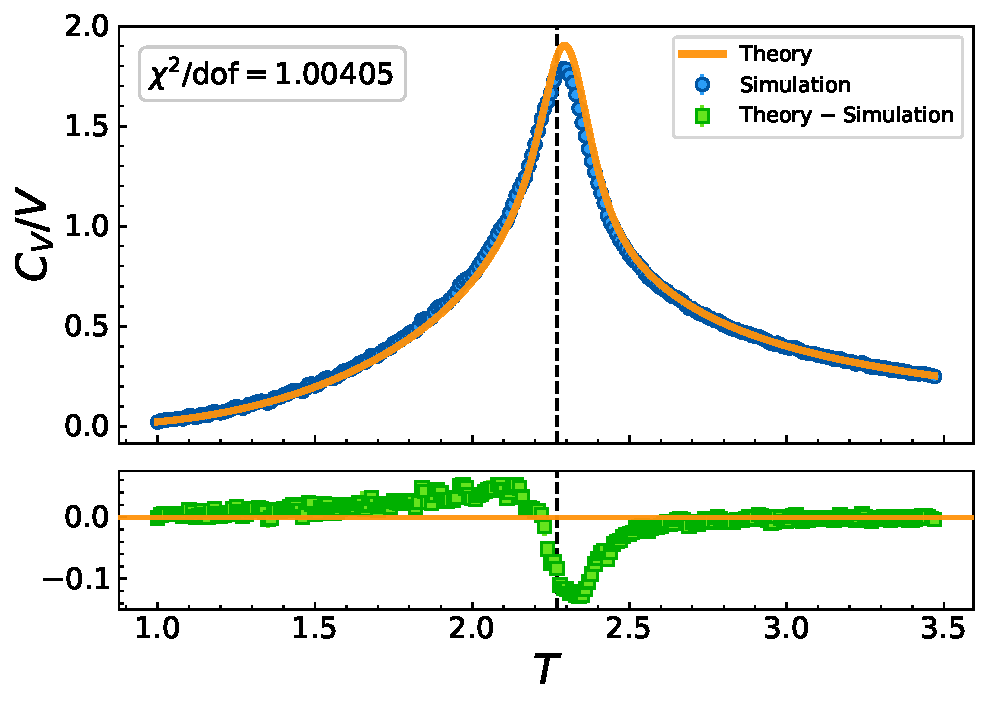
\includegraphics[width=0.8\textwidth]{kauffman_Cv_statistics}
 \caption{Comparison of the worm Monte Carlo computation of the specific heat
		$C_v$ versus temperature and the exact results using the formula
		in~\cite{bkaufman}, for an $L=32$ lattice. Note that $\chi^2 / \text{dof}$
		represents the reduced chi-squared statistic. It can be seen that the
		agreement is excellent, except for a slight deviation at the critical
		temperature, where Monte Carlo algorithms tend to face difficulties with
		critical slowing down.  This is mostly addressed with the worm algorithm,
		in terms of having a dynamical scaling exponent that is zero rather than
		two, but there is (as can be seen), still a residual suppression of
		fluctuations in the immediate vicinity of $T_c$.}%
	 \label{Kcompare}
\end{figure}
%
\subsection{Conjecture About \texorpdfstring{$\lambda_{\max}$}{λmax}}%
\label{ssec:conjecture}
Using the Monte Carlo algorithm outlined above, we can calculate the average
number of occupied bonds at a particular temperature by averaging over all
configurations
%
\begin{align}
    \langle N_b\rangle
        &\equiv \frac{1}{N_{\mathrm{configs}}}\sum_{n=1}^{N_{\mathrm{\mathrm{configs}}}} N_b^{(n)}\\
        &= \left\langle \sum_{j=bonds} v_j \right\rangle \\
        &= 2V\langle \mathbf{v}_b\rangle.
    \label{eq:link_avg}
\end{align}
%
From this, we have that
%
\begin{equation}
    \langle \mathbf{v}_b\rangle = \frac{\langle N_b\rangle}{2V},
\end{equation}
%
where we have defined $\langle \mathbf{v}_b\rangle$ to be the average
occupation of bonds, $N_b^{(n)}$ to be the number of occupied bonds in the
$n$-th configuration, and we have used Eq. (\ref{eq:link_sum}) in the second
line.
%
If we consider graphs with no self-intersections,
%
\begin{equation}
    \sum_{j=bonds} v_j = \sum_{j=sites} v_j.
    \label{bonds_equal_sites}
\end{equation}
%
For small $\beta$ (high $T$) this can be a good approximation,
%
\begin{align}
    \left\langle \sum_{j=bonds} v_j \right\rangle &\simeq \left\langle
    \sum_{j=sites} v_j\right\rangle\Longrightarrow\\
    \langle\mathbf{v}_b\rangle &\simeq \frac{1}{2}\langle\mathbf{v}_s\rangle
    \label{avg_bonds_equal_sites}
\end{align}
%
This agrees with our intuition, that the average image $\langle
\mathbf{v}\rangle$ should resemble a ``tablecloth'', where the site pixels are
twice as dark as the link pixels.
%
This can be seen clearly in Fig.~\ref{fig:average_image}.
%
\begin{figure}[htpb]
    \centering
    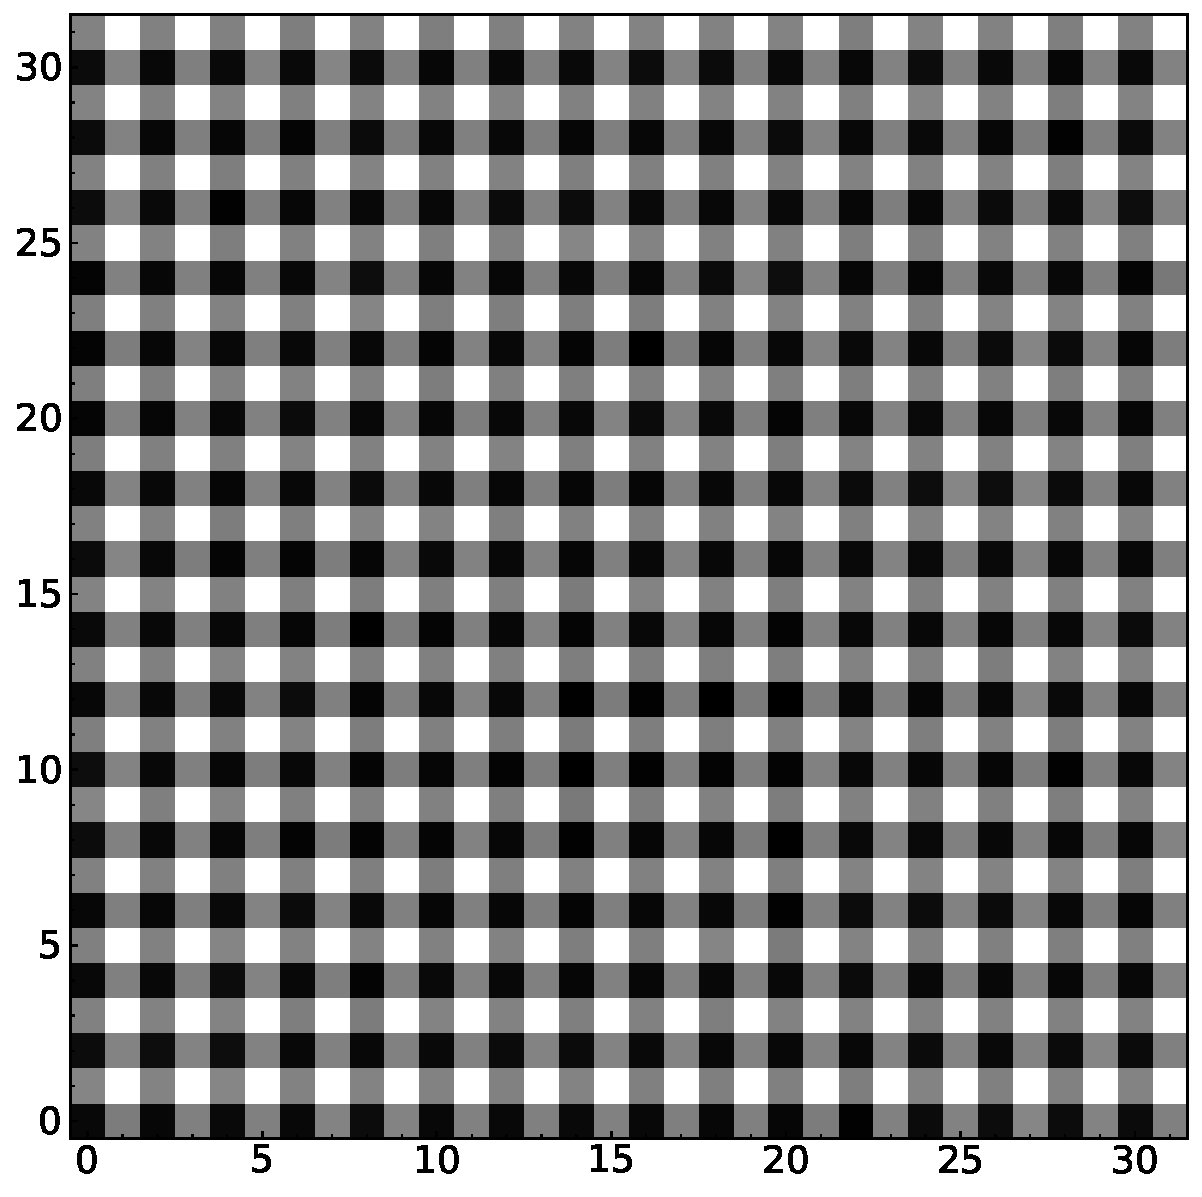
\includegraphics[width=0.8\textwidth]{average_image_16}
    \caption{Average image $\langle \mathbf{v}\rangle$ calculated for the
        $L = 16$ lattice at $T = 2.0$, illustrating the
        tablecloth-like appearance.}%
\label{fig:average_image}
\end{figure}
%
For a general graph, a link is shared by two sites (its endpoints), whereas a
site can be shared by either $0$, $2$, or $4$ bonds.  
%
If the site is shared by two bonds, it is only visited once, denoted
$sites^{(1)}$, and if it is shared by four bonds, it is visited twice, denoted
$sites^{(2)}$.
%
This allows us to break up the sum over bonds into two terms
%
\begin{equation}
    \sum_{j=bonds} v_j = \frac{2}{2}\sum_{j=sites^{(1)}} v_j
        + \frac{4}{2} \sum_{j=sites^{(2)}} v_j
\end{equation}
%
Rearranging and taking averages gives
%
\begin{align}
    \left\langle \sum_{j=sites^{(1)}} v_j \right. 
    + \left. \sum_{j=sites^{(2)}} v_j \right\rangle
    &=\left\langle \sum_{j=bonds} v_j - \sum_{j=sites^{(2)}} v_j \right\rangle\\
    &= \left\langle \sum_{j=sites} v_j\right\rangle\\
    &= V\left\langle \mathbf{v}_s\right\rangle\\
    & = \left\langle \sum_{j=bonds} v_j \right\rangle - \left\langle
        \sum_{j=sites^{(2)}} v_j \right\rangle\\
    &= 2V \langle\mathbf{v}_b\rangle - \left\langle
        N_{sites^{(2)}}\right\rangle\quad\Longrightarrow\\
    \frac{\left\langle N_{sites^{(2)}}\right\rangle}{V} &=
        2\langle\mathbf{v}_b\rangle - \langle \mathbf{v}_s\rangle.
\end{align}
%
We can rewrite the last equation using (\ref{eq:link_avg})
%
\begin{equation}
    \langle \mathbf{v}_s \rangle= \frac{\langle N_b\rangle}{V} - \frac{\langle
        N_{sites^{(2)}}\rangle}{V}.
\end{equation}
%
This suggests that a departure from a perfect tablecloth ($\langle
\mathbf{v}_s\rangle = 2\langle \mathbf{v}_b\rangle$) contains information.
%
% \begin{equation} C = (V - \langle V\rangle)^T(V - \langle V\rangle)
% \end{equation}
%
%
% with entries,
%
Another useful construct is the \emph{covariance matrix},
%
\begin{align}
    C_{ij} &=
    \left\langle\left(v_i -\langle \mathbf{v}\rangle_i\right)
    {\left(v_j -\langle \mathbf{v}\rangle_j\right)}^{T}\right\rangle\\
        &= \frac{1}{N_{\mathrm{configs}}}\sum_{n=1}^{N_{\mathrm{configs}}}
        {\left(v_i^{(n)} -\langle \mathbf{v}\rangle_i\right)}
        {\left(v_j^{(n)} -\langle \mathbf{v}\rangle_j\right)}^{T},
\label{covariance_matrix}
\end{align}
%
where we have defined $v_k^{(n)}$ to be the grayscale value of the $k$-th pixel
in the $n$-th sample configuration, and $\langle \mathbf{v}\rangle_k$ is the
average grayscale value of the $k$-th pixel over the set of configurations.
% whose significance will become apparent in later sections.

At some fixed temperature, the covariance matrix, $C \in
\mathbb{R}^{N_{\mathrm{configs}}\times4L^2}$, where $N_{\mathrm{configs}}$ is
the number of sample configurations (images), with each configuration flattened
into a vector of length $4L^2$.
%
We can then perform a singular value decomposition (SVD) on the covariance
matrix,
%
\begin{equation}
    C = W\Lambda W^{T}
    \label{svd}
\end{equation}
%
where $W$ is a $4L^2\times 4L^2$ matrix whose columns ($\mathbf{w}_k$) are the
eigenvectors of $C$, and $\Lambda$ is the diagonal matrix of the absolute value
of the eigenvalues $\lambda^{(k)}$ of $C$, arranged in decreasing order.
%
Without loss of generality, we can assume that the eigenvectors $\mathbf{w}_k$
are real and normalized such that $\mathbf{w}_k^{T} \mathbf{w}_k = 1$.
%
Thus, we can write
%
\begin{align}
    C \mathbf{w}_k &= \lambda^{(k)} \mathbf{w}_k\\
    \mathbf{w}_k^{T} C \mathbf{w}_k &= \lambda^{(k)}
\end{align}
%
For our purposes, we are interested in the first principal component, with
eigenvalue $\lambda^{(1)} \equiv \lambda_1$ and corresponding eigenvector
$\mathbf{w}_1$.
% \equiv \mathbf{w}^{max}$.

We conjectured that the first principal component, $\mathbf{w}_1$ of the
covariance matrix $C$ is directly proportional to the average worm
configuration (image) $\langle \mathbf{v} \rangle$, i.e.
%
\begin{equation}
    \mathbf{w}_1 \propto \langle \mathbf{v}\rangle.
    \label{conjecture}
\end{equation}
%
From our results in~\ref{configs_as_images}, we can write
%
\begin{align}
    % \sum_j \langle \mathbf{v}_j \rangle \langle \mathbf{v}_j \rangle =
    \langle \mathbf{v}\rangle^2
    &= \langle \mathbf{v}\rangle^{T} \langle \mathbf{v}\rangle \\
    &= 2V\bondavg^2 + V \siteavg^2.
    % 2V\langle \mathbf{v}_b \rangle^2 + V \langle \mathbf{v}_s\rangle^2
\end{align}
%
This suggests that
%
\begin{equation}
    \mathbf{w}_1 = \frac{\langle \mathbf{v}\rangle}{\sqrt{(2\bondavg^2 +
    \siteavg^2)V}}.
\end{equation}
%
Moreover, we can write
%
% &\quad\quad\quad-\left(2V\bondavg^2+V \siteavg^2\right)\bigg\}\\
% &\quad\quad\quad-V\left(2\bondavg^2+\siteavg^2\right)\bigg\}\\
\begin{align}
  \sum_i {\left(v_{i}^{(n)} - \langle\mathbf{v}\rangle_i \right)}
    \langle\mathbf{v}\rangle_{i}
       &= {\bondavg\sum_{j=bonds}v_{j}^{(n)}
         +\siteavg\sum_{j=sites}v_j^{(n)}
         -\left(2V\bondavg^2+V \siteavg^2\right)}\\
       &= \bondavg N_b^{(n)}+\siteavg N_{s}^{(n)}
         -V{\left(2\bondavg^2+\siteavg^2\right)}\\
       &= \bondavg{\left(N_b^{(n)}-\langle N_b\rangle\right)}
         +\siteavg{\left(N_s^{(n)}-\langle N_s\rangle\right)}\\
       &\equiv \bondavg \Delta_{N_b}^{(n)} + \siteavg \Delta_{N_s}^{(n)}.
\end{align}
%
From this, we can extract a relationship between the eigenvalue corresponding
to the first principal component, $\lambda^{(1)}$ and the fluctuations
$\Delta_{N_b}$ and $\Delta_{N_s}$,
%
\begin{align*}
    \mathbf{w}_1^{T} C \mathbf{w}_1
        &= \lambda^{(1)}\\
        &= \frac{1}{N_{\mathrm{configs}}}\sum_{n=1}^{N_{\mathrm{configs}}} \frac{%\bigg[
          {\left[\bondavg \Delta_{N_b}^{(n)}\right]}^2 + 2\bondavg \siteavg \Delta_{N_b}^{(n)} \Delta_{N_s}^{(n)}
        + {\left[\siteavg \Delta_{N_s}^{(n)}\right]}^2 }{2\bondavg^2 + \siteavg^2}
        % &\quad\quad\quad\quad\quad\quad\quad\quad\quad
\end{align*}
%

Now, if we consider the high temperature approximation where sites only have
single visits (no self-intersections), $\siteavg \simeq 2\bondavg$, $\langle
N_s\rangle \simeq \langle N_b\rangle$, and $\Delta_{N_b} \simeq \Delta_{N_s}$,
we have that $2\bondavg^2 + \siteavg^2 \simeq 6\bondavg^2$ and
%
%
\begin{align}
    \lambda_1 &\simeq \frac{\bondavg^2}{N_{\mathrm{configs}}}\frac{9}{6\bondavg^2}
    \sum_{n=1}^{N_{\mathrm{configs}}} {\left(\Delta_{N_b}^{(n)}\right)}^2 \\
    &= \frac{3}{2}\frac{1}{N_{\mathrm{configs}}}\sum_{n=1}^{N_{\mathrm{configs}}}
    {\left(\Delta_{N_b}^{(n)}\right)}^2 \\
    &= \frac{3}{2}\left \langle \Delta_{N_b}^2 \right\rangle.
    \label{eq:eigval_delta_Nb2}
\end{align}
%

A justification for making this approximation can be seen in
Fig.~\ref{fig:twice_visited_sites_ratio}. 
%
%
\begin{figure}[htpb]
  \centering
  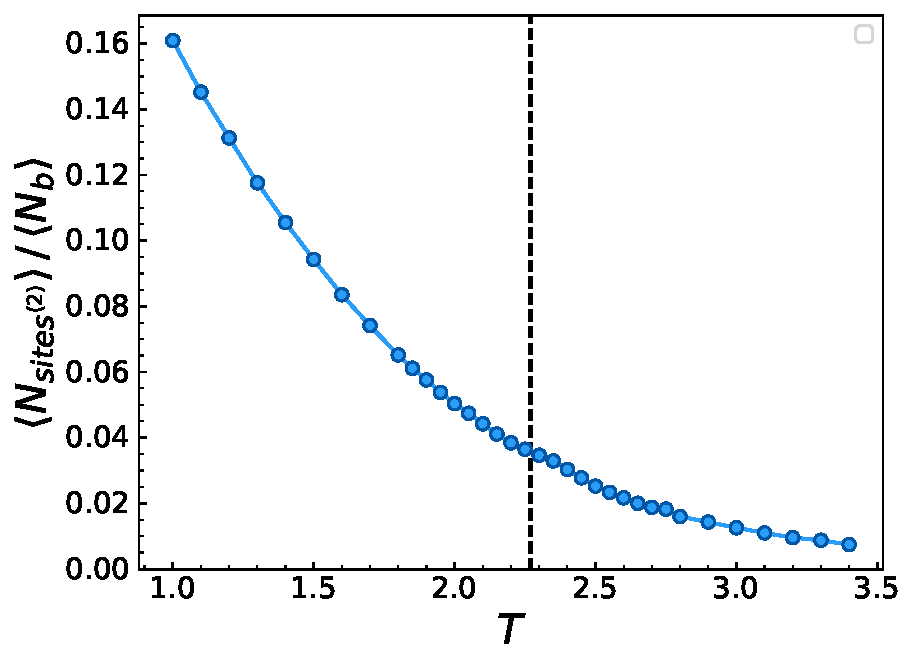
\includegraphics[width=0.8\textwidth]{twice_visited_sites_ratio}
  \caption{Ratio of the number of twice visited sites $\langle
    N_{sites^{(2)}}\rangle$ to the average number of bonds $\langle N_b\rangle$
    versus temperature, for the $L=32$ lattice. This clearly justifies our
    approximation $\siteavg \simeq 2\bondavg$, where we ignore the contribution
  from twice visited sites.}%
\label{fig:twice_visited_sites_ratio}
\end{figure}
%
%

\subsection{Illustration of Alternate Blockings}%
\label{subsec:altb}
In Fig~\ref{fig:alt_blockings} we consider the alternative blocking procedures:
$1 + 1 \rightarrow 1$ and $1 + 1 \rightarrow 2$.
%
% \begin{widetext}

\begin{figure}[htpb]
    \centering
    \subfigure[ $1 + 1 = m$]{%
        \centering
        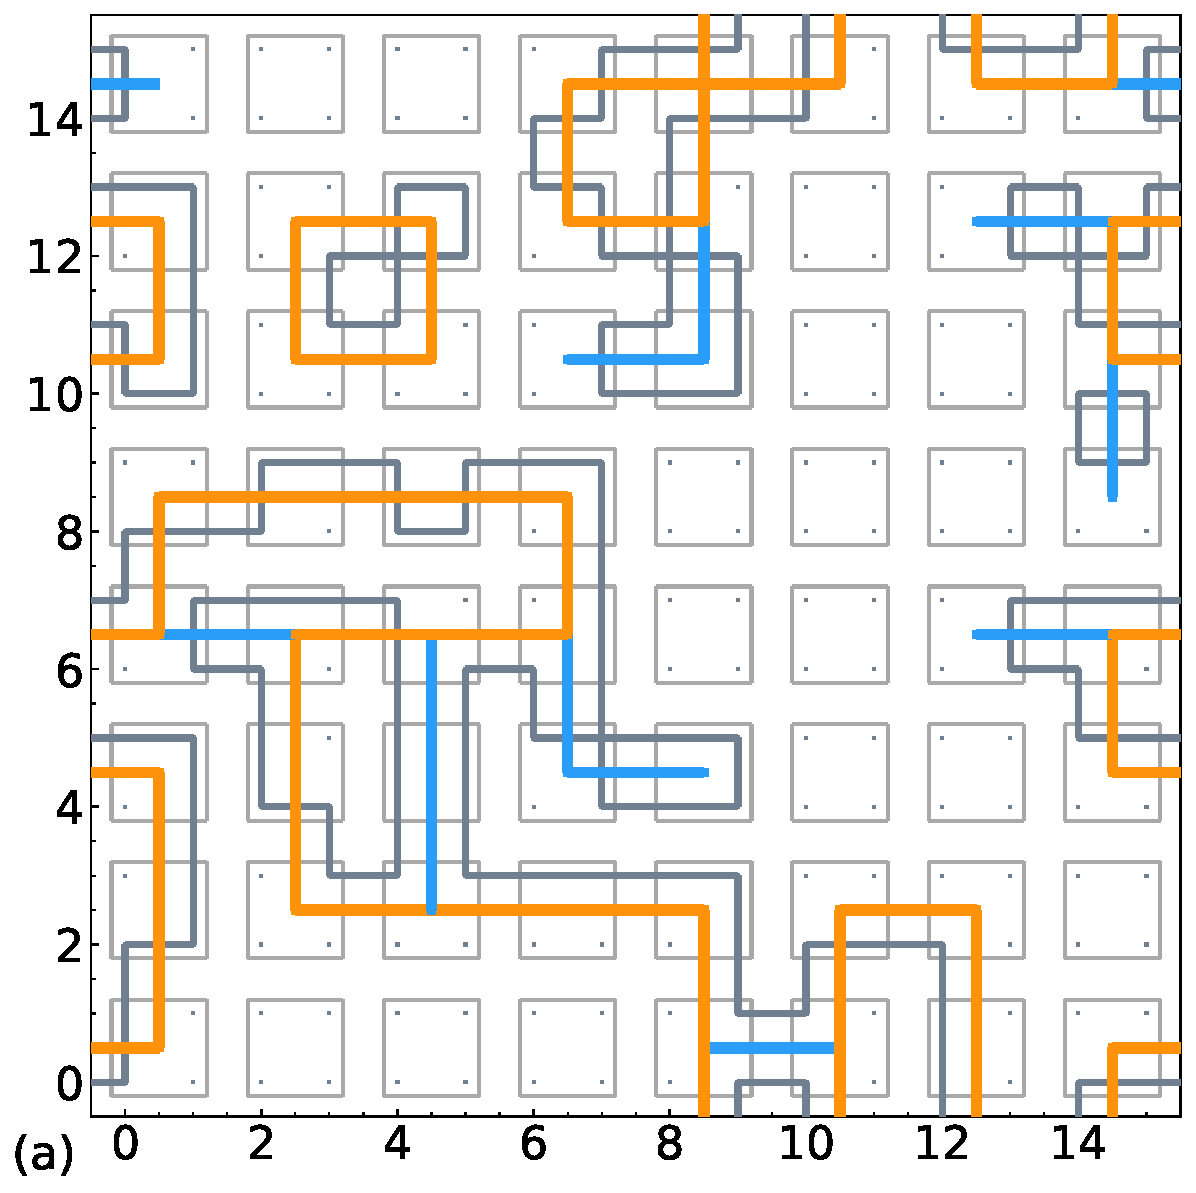
\includegraphics[width=0.30\textwidth]{worm_configuration_16_blocked11m}\label{fig:blocked_exact2}
    }\hfill
    \centering
    \subfigure[ $1+1\rightarrow 1$]{%
        \centering
        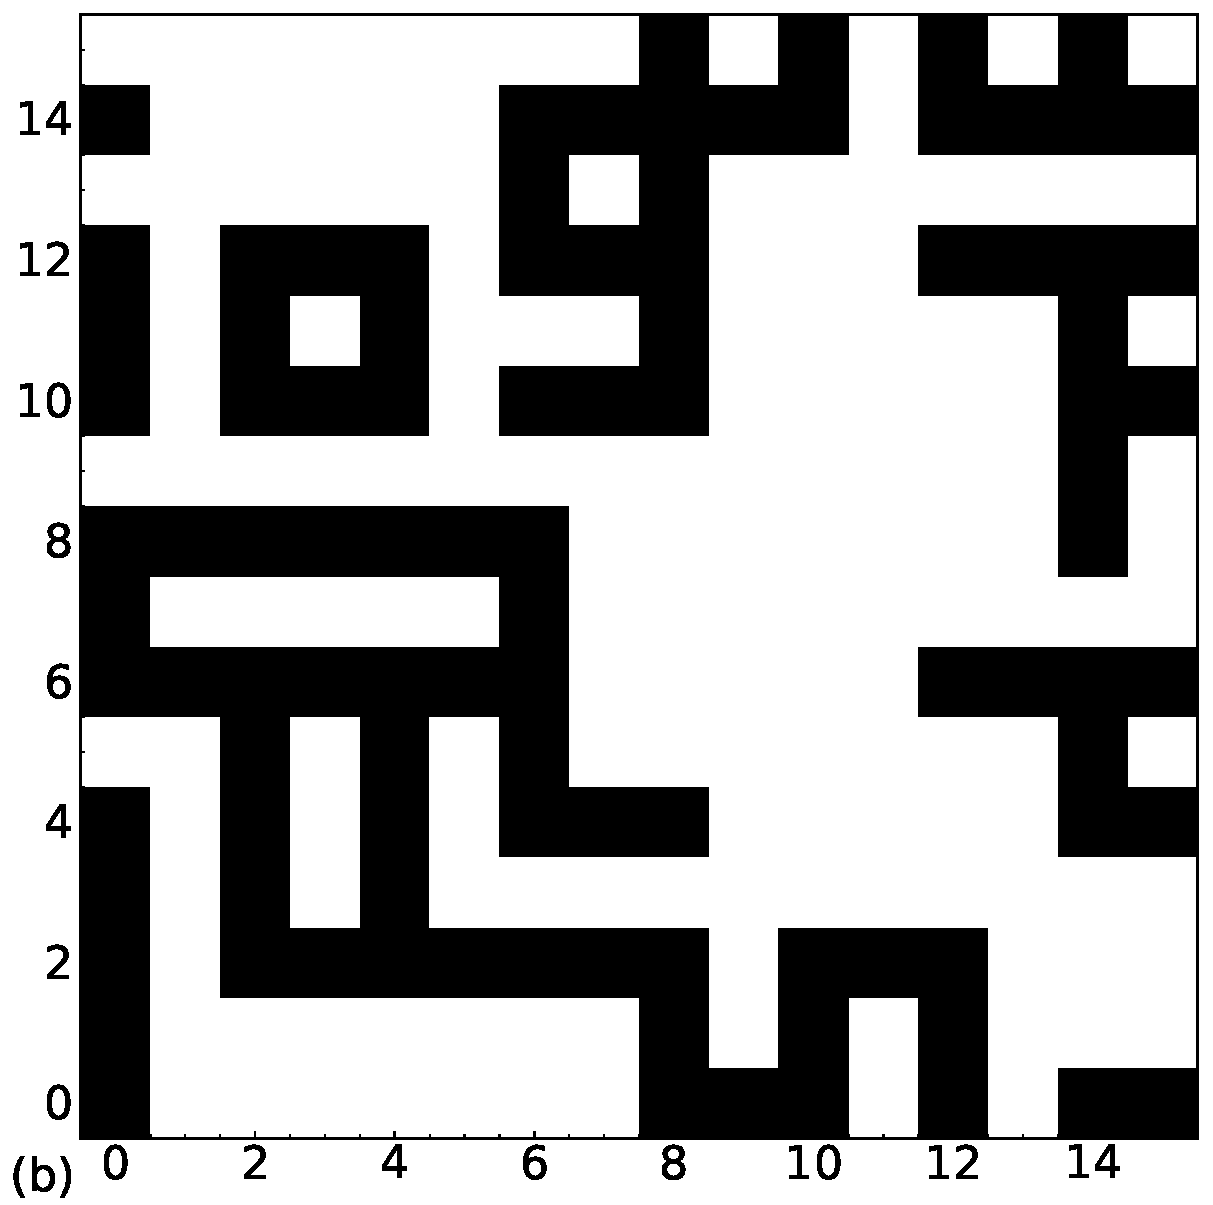
\includegraphics[width=0.30\textwidth]{worm_configuration_16_blocked111_image}\label{fig:blocked_exact1_pca}
    }\hfill
    \subfigure[ $1+1\rightarrow 2$]{%
        \centering
        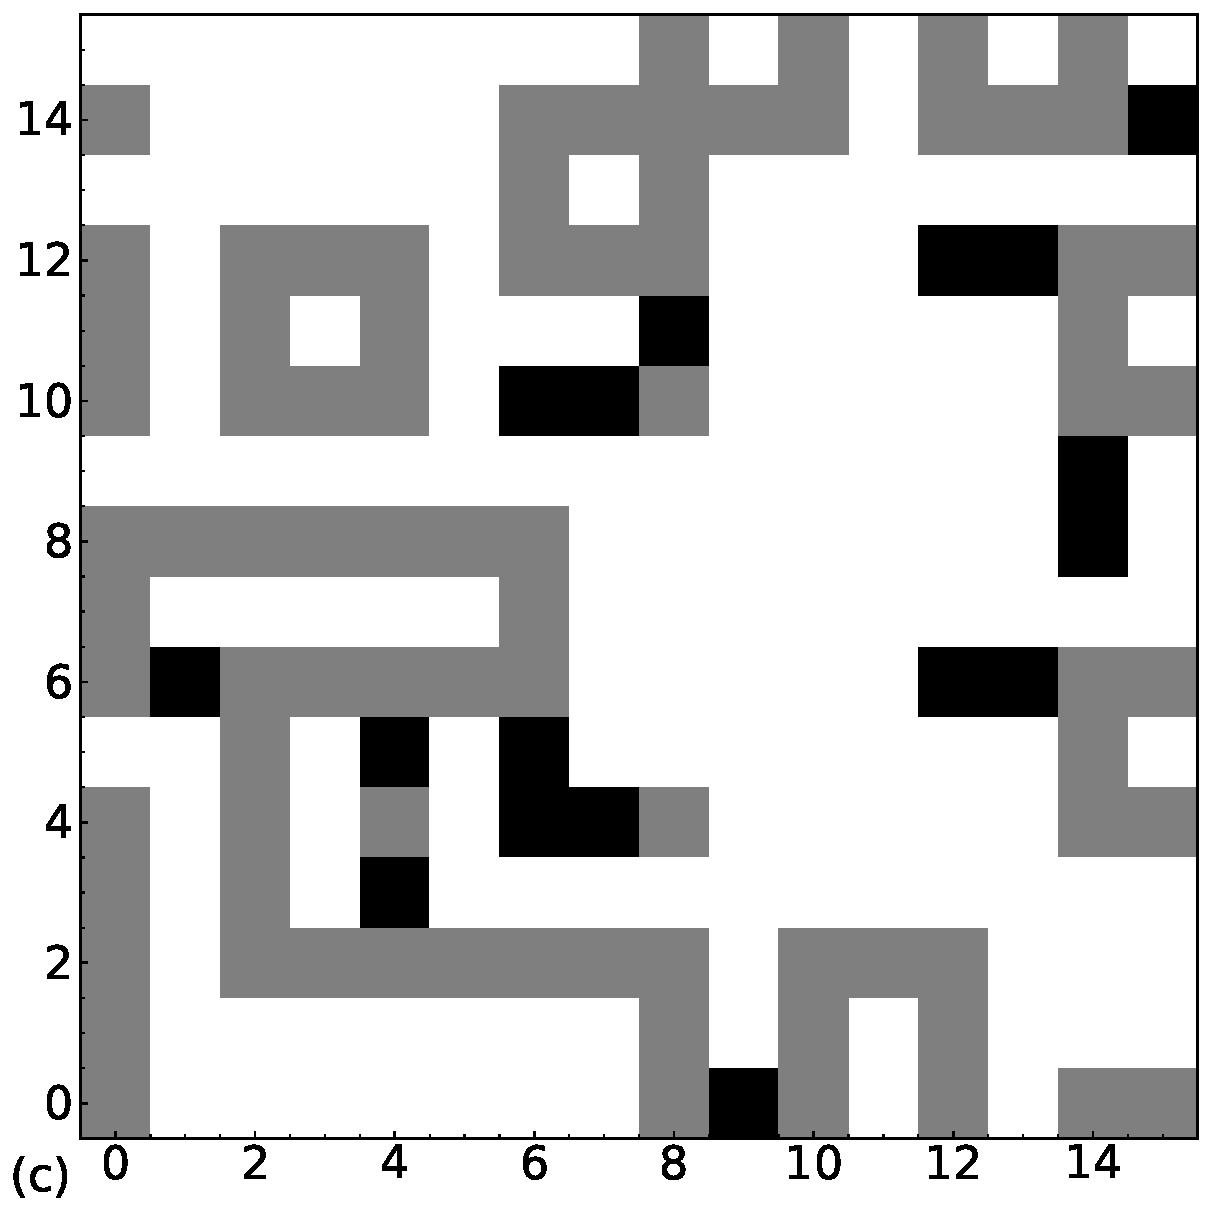
\includegraphics[width=0.30\textwidth]{worm_configuration_16_blocked112_image}\label{fig:blocked_exact2_pca}
    }\hfill
    \caption{Example of the different coarse-graining (``blocking'') procedures
      applied to a sample worm configuration generated at $T = 2.0$. Note that
      in (\ref{fig:blocked_exact2}) $m \in \{1, 2\}$, and double bonds are
      represented by blue lines.  (\ref{fig:blocked_exact1_pca}),
      (\ref{fig:blocked_exact2_pca}), illustrate the results of applying
      different weights to the so-called ``double bonds'' in the images
      representing a blocked configuration. Note that in
      (\ref{fig:blocked_exact1_pca}) $1+1\rightarrow 1$, double bonds are given
      the same weight as single bonds, and in (\ref{fig:blocked_exact2_pca})
    $1+1\rightarrow 2$, double bonds are given twice the weight as single
  bonds, appearing twice as dark.}\label{fig:double_bond_weights}%
\label{fig:alt_blockings}
\end{figure}
%
% \end{widetext}
%
\section{Possible Applications: From Images to Loops}%
\label{sec:cifar} 
Having better understood how these RG transformations can be used to describe
the 2D Ising model near criticality, we began to look for possible applications
to real-world datasets.
%
For our analysis, we used the CIFAR-10~\cite{Krizhevsky09} image set consisting
of $60,000$ $32\times32$ color images in 10 classes.
%
First, each of the images were converted to a grayscale with pixel values in
the range $[0, 1]$.
%
Next, a grayscale cutoff value was chosen so that all pixels with values below
the cutoff would become black, and pixels above the cutoff would become white,
resulting in images consisting entirely of black and white pixels.
%
Finally, each of these images were converted to `worm-like' images by drawing
the boundaries separating black and white collections of pixels.
%
An example of these preprocessing steps are illustrated in
Fig.~\ref{fig:CIFAR10_preprocessing}.
%
\begin{figure*}[htpb]
 \centering
 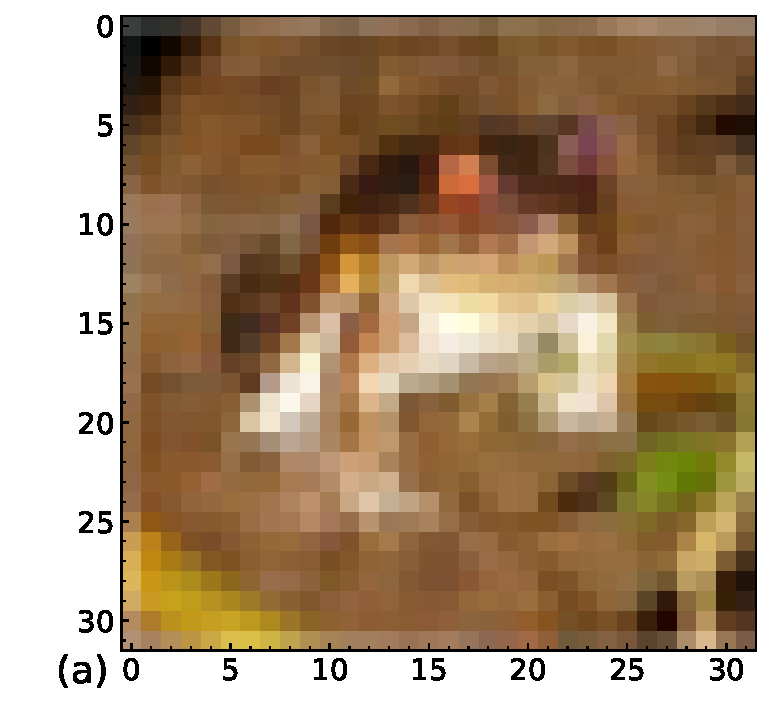
\includegraphics[width=0.32\textwidth]{CIFAR10_image0}
 \hspace{1.5cm}
 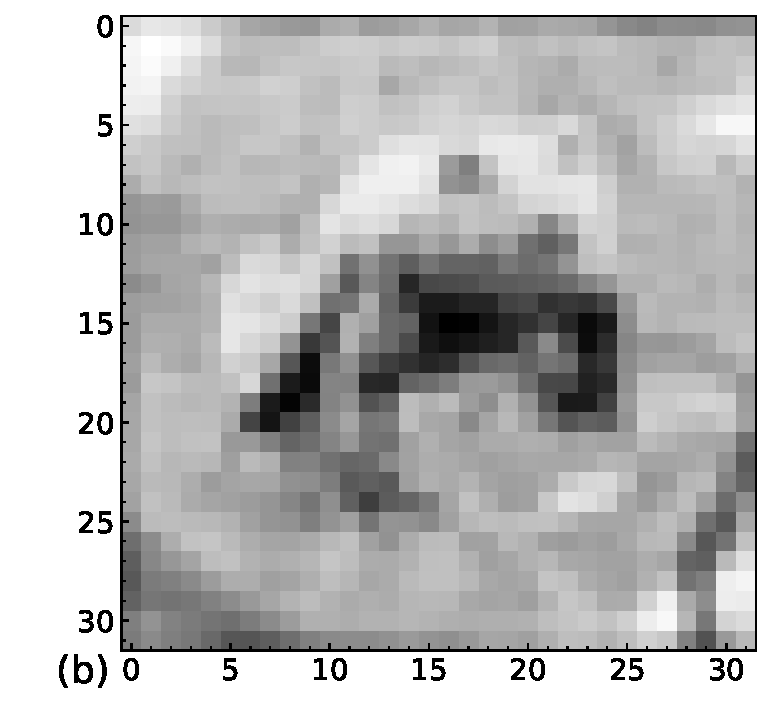
\includegraphics[width=0.32\textwidth]{CIFAR10_grayscale_image0}
 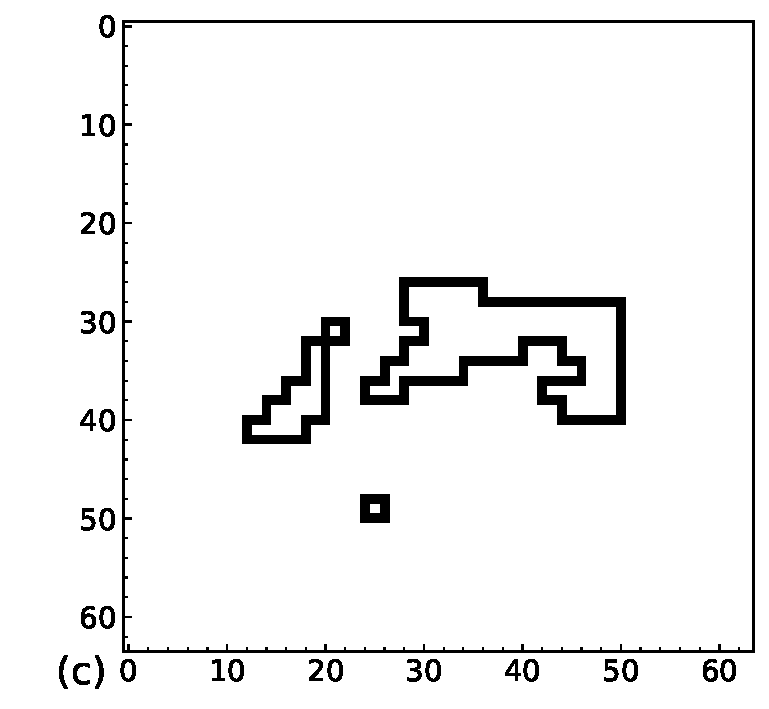
\includegraphics[width=0.32\textwidth]{CIFAR10_boundary_image0_025}
 \hfill
 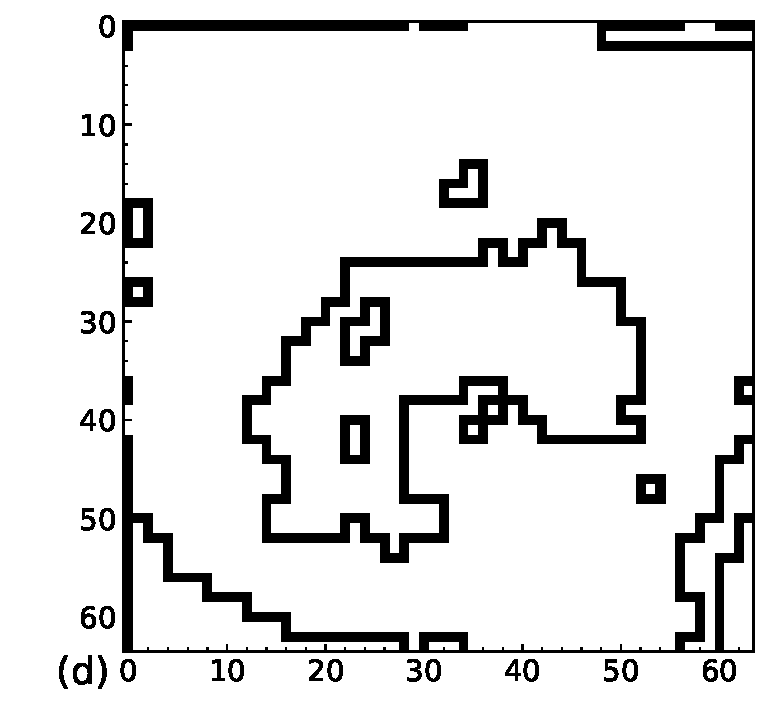
\includegraphics[width=0.32\textwidth]{CIFAR10_boundary_image0_05}
 \hfill
 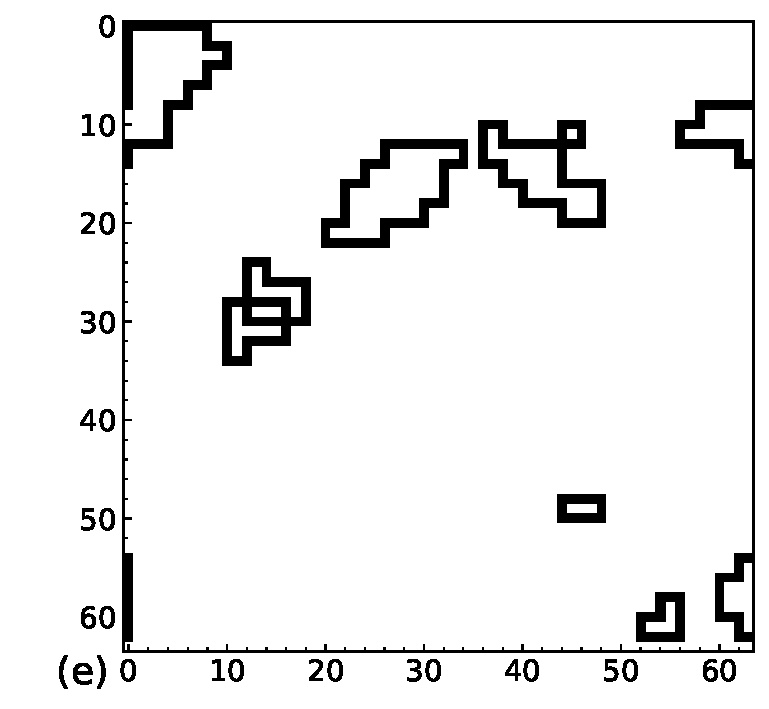
\includegraphics[width=0.32\textwidth]{CIFAR10_boundary_image0_075}
 \caption{Example of preprocessing steps for converting CIFAR-10 images to
		`worm-like' images, illustrating the resulting image for different values
		of the grayscale cuttoff. (a) Original image from CIFAR-10 dataset. (b)
		Image converted to grayscale.  (c) Resulting image from cutoff values of
		$0.25$, (d) $0.5$, and (e) $0.75$.}%
\label{fig:CIFAR10_preprocessing} 
\end{figure*}
%
%
This process was carried out on a mini-batch consisting of 500 randomly
selected images from the CIFAR-10 image set.
%
For each image in our mini-batch, we calculated $\langle N_b\rangle$ and
$\langle \Delta_{N_b}^2\rangle$ over a range of grayscale cutoff values in $[0,
1]$ in steps of $0.02$.
%
Each of these images were then iteratively blocked using the $(1 + 1
\rightarrow 0)$ blocking procedure described in Sec.~\ref{sec:trg}, calculating
$\langle N_b\rangle$ and $\langle \Delta_{N_b}^2\rangle$ for each successive
blocking step, as shown in Fig.~\ref{fig:CIFAR10_bond_stats}.
%
\begin{figure*}[htpb]
    \centering
    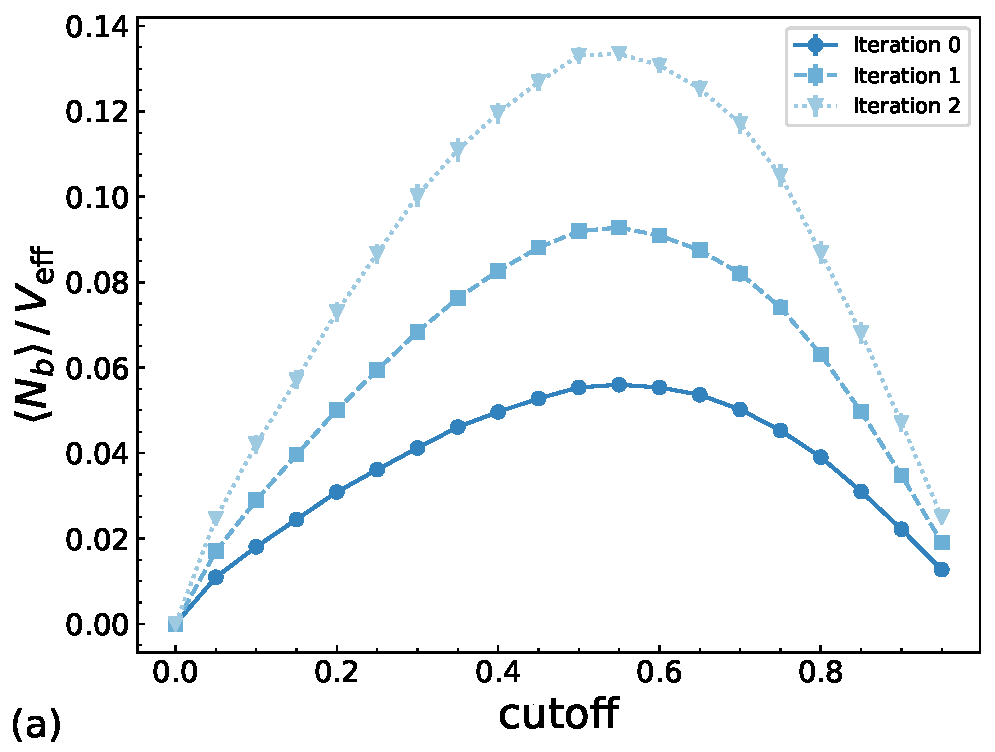
\includegraphics[width=0.49\textwidth]{Nb_avg_vs_cutoff_CIFAR10.pdf}
    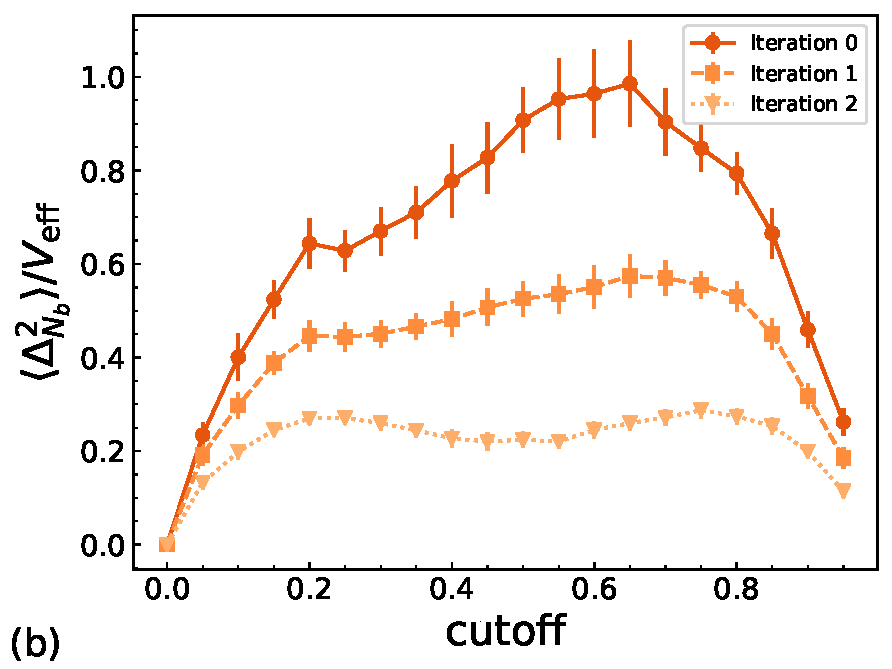
\includegraphics[width=0.49\textwidth]{delta_Nb_avg_vs_cutoff_CIFAR10.pdf}
    \caption{$\langle N_b\rangle$ and $\langle \Delta_{N_b}^2\rangle$ vs.\
    grayscale cutoff value for 500 randomly chosen images from the CIFAR-10
  dataset.}%
\label{fig:CIFAR10_bond_stats}
\end{figure*}
%
Immediately we see that there is no identifiable low temperature phase, and
that for cutoff values near both $0$ and $1$, we obtain images which are mostly
empty, similar to the high temperature configurations obtained from the worm
algorithm.
%
This suggests that there is no such notion of criticality (as characterized by
the abrupt transition from a low to high temperature phase) like we found for
the two-dimensional Ising model.

\section{Conclusions}
In summary, we have motivated, constructed and applied a
RG transformation to sets of worm configurations at various temperature.
%
This transformation is approximate and the coarse-grained configurations are
themselves worm configurations.
%
This allows multiple iterations.
%
We monitored the bond density at successive iterations and compared them with a
two-state TRG approximation.
%
We found clear similarities in the low-temperature side, where data collapse is
observed for both procedures when the distance to the critical point is
rescaled at each iteration.
%
In the high-temperature phase, only the TRG approximation shows good data
collapse. 

Can the procedure developed here be applied to the boundary of arbitrary sets
of images as illustrated in the introduction?
%
The gray cutoff could be used as a tunable parameter.
%
However, in the limiting cases of a zero (one) gray cutoff we have uniform
black (white) images which are both similar to the high-temperature phase, and
we do not expect a phase transition.
%
Applications to the CIFAR dataset are discussed in Section~\ref{sec:cifar} and
confirm this point of view. 

RG methods have been considered for assisting in image recognition~\cite{16712,
0305-4470-35-37-201,1997PhLA..227..319H}.
%
By mapping from fine to coarse in several ways, such as the $1 + 1\rightarrow
0$ and $1 + 1\rightarrow 1$ in our approach, one begins to see how the inverse
process might go in replacing a degraded image with a higher resolution
reconstruction.
%
The physics of defining RG transformations and quantifying scheme dependence
then guides such reconstructions using physical principles, which are expected
to be embedded into real world image characteristics due to principles of
universality.

It should be noted that the TRG procedure is often considered as a ``local
update'' of the tensor.
%
A more sophisticated approach consists of using the standard recursion to
provide an environment for subsequent
updates~\cite{PhysRevLett.103.160601,PhysRevB.86.045139}.
%
An environment tensor $E$ is propagated backward from the coarse to the fine
scale.
%
An improved version of the initial iteration can then be performed in an
environment.
%
This forward-backward procedure can be repeeated and is very reminiscent of the
procedure proposed by Hinton and Salakhutdinov~\cite{Hinton504} in the context
of image recognition.

A better understanding of RG concepts in machine learning could enhance physics
discovery, especially in the context of simulation and modeling of physical
systems at a fundamental level~\cite{Shanahan:2018vcv}.
%
The general idea is to render computational tools ``smart,'' i.e., that they
would learn features and patterns without the intervention of a human
``assistant,'' and would, in the best possible scenario, guide the direction of
further simulations.
%
This could accelerate and deepen the process of understanding and
characterizing the complex systems that are deemed important in pure and
applied physics.
\end{document}
